
\chapter[Background]{Background}
\label{chapter:backround}
\section{Environmental Sound Classification}
\label{chapter:backroundIntroESC}
Environmental sound classification (ESC) is the task of detecting and classifying sounds that originate from  human or non-human activities, such as sound emanated by the passing of a car, a dog barking, or sound produced by the drops of rain. Environmental sound classification is a general term and includes many fields such as sound event detection (SED) \cite{mesaros2021sound, heittola2013context}, acoustic scene classification (ASC) \cite{abesser2020review, mesaros2016tut}, bird sound detection \cite{kahl2017large, adavanne2017stacked} and many more \cite{turpault2020improving, lavner2016baby, pandeya2018domestic, salamon2015unsupervised, piczak2015environmental}. 

Recently, ESC has been a hot topic for researchers. This increase of interest in ESC is due to the introduction of neural networks and their application in image and speech recognition \cite{choi2016dnn, perez2017effectiveness, deng2013new} and partly because of competitions organized \cite{mesaros2017dcase, mesaros2019sound, mesaros2017detection, BOJER2020} to improve the performance in the recognition of daily life sound events. Another reason for this interest is the increasing potential application of ESC. These applications of sound event recognition are spread in various domains  such as wildlife monitoring, traffic analysis, industrial noise control, smart homes, and smart cities. For example, bird sounds and wildlife sound recognition \cite{stowell2016bird} can be used for the preservation of wildlife in forests, breakage and gunshot detection \cite{lim2017rare} for security purposes, activity detection in smart homes, fall detection for elderly persons\cite{adnan2018fall}. The use of advanced machine learning techniques and new technologies like deep learning allows us to improve the accuracy and robustness of the classification process, making it more reliable in real-world settings. The detection and recognition of the events in surroundings and their use to ameliorate life experiences and improve automation in different applications.

Environment sound classification systems are composed  of sound recording, sound representation, and classifying systems. The sound recording is the phase where different sounds are recorded using a digital microphone and a database is created. The second step, after obtaining audio recordings and labels, is processing the sound recordings for the classification stage. This processing stage is generally called sound representation or feature extraction. In this stage, the audio recording is processed, and depending on the process the sound is manipulated in other domains, for example, the transformation from a one-dimensional time domain to a two-dimensional time-frequency domain. In this stage, the sound is represented as an image, further discussed in detail in the next section. 

The last stage of the ESC system is the classification stage, where the sounds after processing are sent to the classifier with the target label during the learning stage, and in the testing stage only the processed input is applied and the label associated with the sound is obtained. This is the most important stage in the ESC system and hence the most difficult. To classify sounds, several methods have been studied in the past. Machine learning algorithms have performed better on the task of classifying sounds and recently neural networks are being used to classify sounds. The neural networks are part of machine learning algorithms that are based on the neuron in the brain cell. Neural networks are quite handy in the task of classifying images and sounds. Nowadays, machine learning models such as CNN, RNN, and LSTM are considered the first choice and state of the art for various tasks including ESC, due to their ability to model complex relationships and non-linear patterns in data, as well as their ability to handle large and high-dimensional data such as sound \cite{DCASE2020Workshop, DCASE2019Workshop, dcase2022, piczak2015environmental}.



\section{Sound Representation / Feature Extraction} 
\label{chapter:backroundSoundRepresentation}
Audio signals are discrete streams of bits when recorded with a digital microphone. These signals are generated by several sources and are recorded in real-life environments or are generated synthetically. The signals are represented in the time domain with changing amplitudes with respect to time. The sequence is the lowest possible method for representing any sound events. However, this lowest level representation is extremely difficult for a machine learning model to learn to which category the sound belongs and performs inferences afterward. To address this issue, often the sounds are converted into a different form of representation which the classifier can learn. This representation of sound derived from the lowest level to a different form is known as features or specifically for audio signals acoustic features. The most common method to extract acoustic features consists of converting the time domain signal into a frequency domain. Signals belonging to the same category often share characteristics in the frequency domain. Another advantage of frequency domain representation is that it is more robust to noise and compact and allows more processing as compared to time domain representation. The number of stages of processing over the time domain signal, to obtain the acoustic features, defines the level of abstraction for the representation of sound. For example, fast Fourier transform-based spectrograms are most commonly used and Mel frequency-based cepstral coefficients (MFCCs) are one abstraction level above the spectrograms. The calculation of MFCCs requires more processing steps in the frequency domain and therefore represents a higher abstraction level as shown in Figure \ref{fig:signalTransformation}. 


\subsection{Steps involved in acoustic feature extraction}
\label{chapter:backroundStepsInvolved}
Fourier transform is the most commonly used method for representing acoustic features in frequency domain\cite{DCASE2020Workshop, DCASE2019Workshop, dcase2022}. The algorithm to apply Fourier transform in short widows is called Short-Time Fourier Transform (STFT) and involves three stages: framing, windowing, and frequency spectrum calculation. To obtain the frequency spectrum through STFT, the inherent property of STFT is assumed i.e. the signal is a sum of stationary sinusoids. Therefore, the audio signal is first divided into short time frames and later the frequency spectrum of each frame is calculated. This stage is known as the framing of the signal. In this scenario we are faced with a trade-off between frequency resolution and time resolution, depending on the length of the frame. The larger the frame length, the higher the frequency resolution and consequently the smaller the time resolution. The length of the frame is selected according to the task at hand. For environmental sound classification, generally, the range between 20 to 50 ms is often adopted \cite{mesaros2021sound}. To have a smooth transition between frames an overlap of 20\% to 50\% of the frame is often selected. This process is done in the windowing operation, where each frame is multiplied with a window function to avoid spectral leakage and discontinuities  at the edge of each frame, which could lead to the corruption of the estimation of the frequency spectrum. Most popular windowing functions such as Hamming, Hann, and Blackman functions are commonly used for window operations in the feature extraction stage. In the next step, the frequency spectrum representation of each frame, subjected to the windowing function, is calculated using a discrete Fourier Transform. Discrete Fourier Transform calculates the spectral information in the window. The frequency and the power related to each frequency are later stacked on a time scale to obtain a time-frequency representation, commonly known as a spectrogram. Transformation is depicted in Figure \ref{fig:signalTransformation}. 


\begin{figure}[htbp]
   \begin{center}
      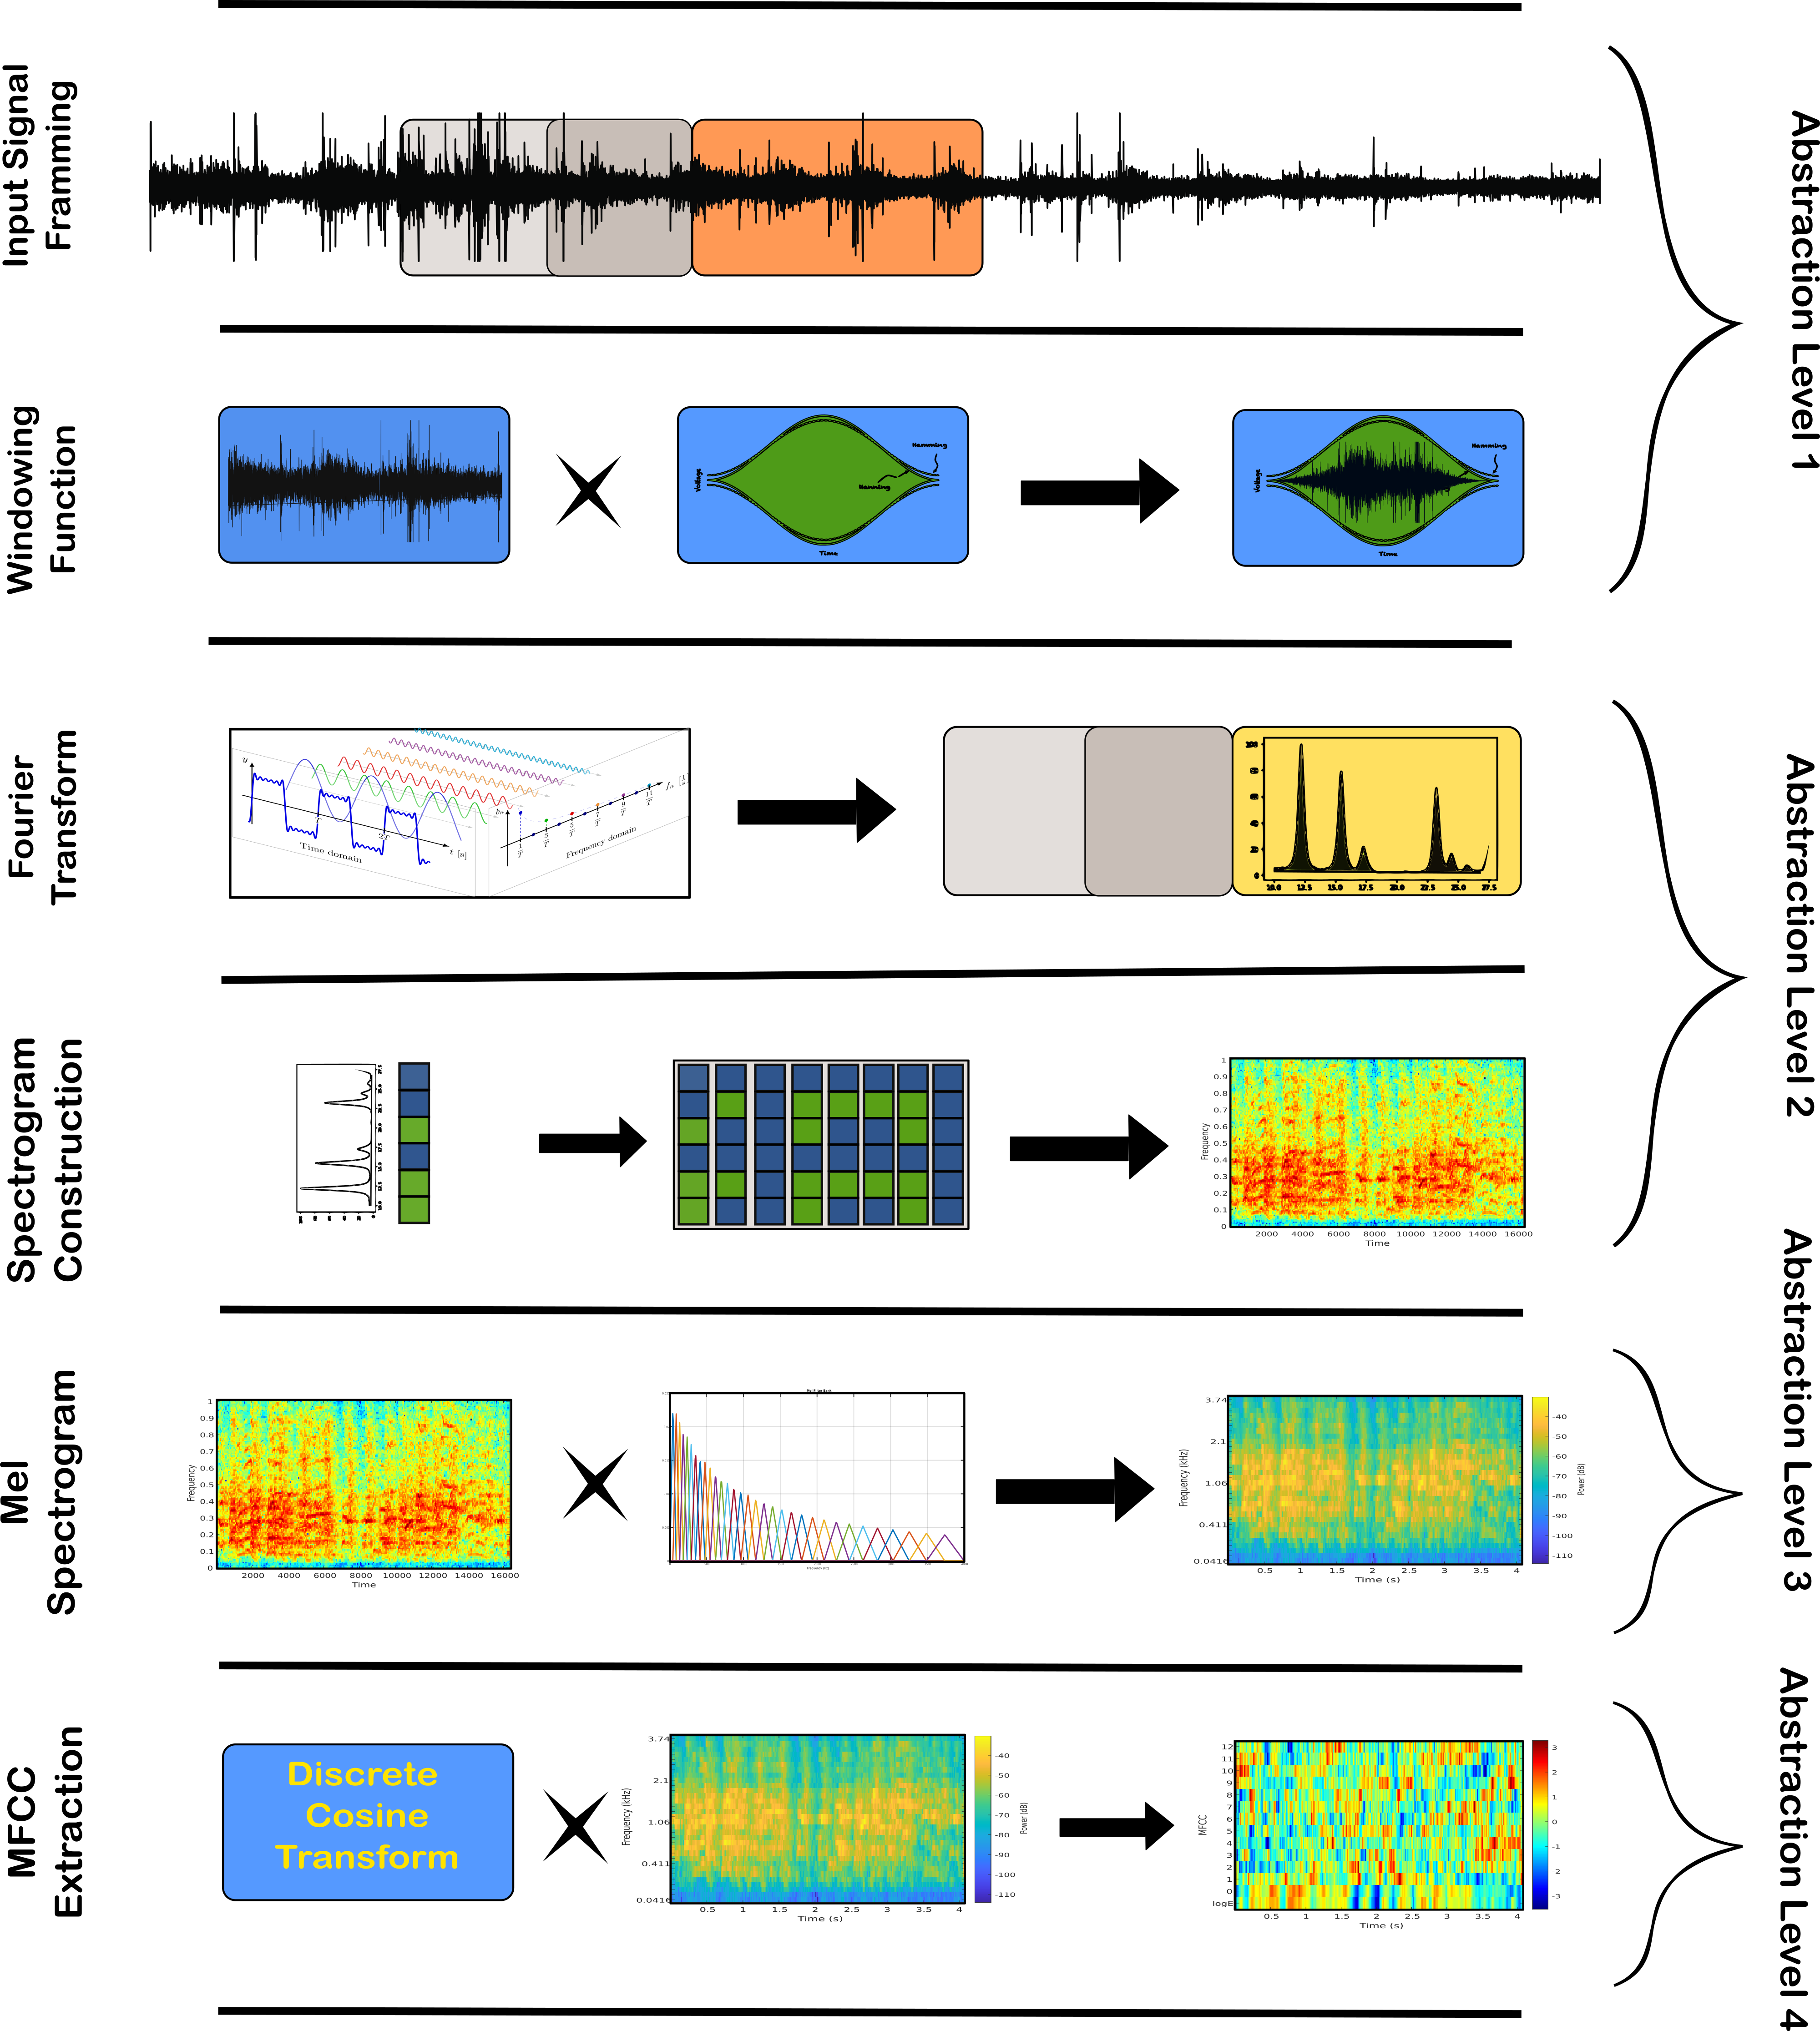
\includegraphics[width=1\linewidth]{Chapitre1/figures/signalTransfromation.png}
   \end{center}
   \caption { Feature extraction stages from an audio signal.}
   \label{fig:signalTransformation}
\end{figure}



\subsection{Spectrogram construction}
\label{chapter:backroundSpectrogramConstruction}
The spectrogram is  a time-frequency feature matrix, obtained by extracting vectors containing spectral components for each consecutive time frame and concatenating them with other vectors according to the time frame of the audio signal. The spectrogram provides the first level of abstraction of the signal as a feature for environmental sound classification. The Fourier transform provides complex values and hence the spectrogram consists of complex values. However, only magnitude is employed and the phase information  of the spectrogram is discarded. The reasoning behind such an operation is that the phase information is deemed to be less informative for the classification system. Sound events mostly demonstrate high energy in a lower frequency range and in time frequency feature representation they dominate the lower frequency components. The logarithm can be employed to compress the dynamic range of the magnitude spectrogram by obtaining the log magnitude spectrogram. 

Spectrograms are considered to be a useful tool for the classification of sound events, as compared to the raw sound signal. Similar to images, spectrograms are multidimensional and this allows the image classification systems developed for image-based classification applicable to sound classification. In addition, as compared to raw audio signals the spectrograms contain more information about the sound event. The spectrogram manifests information in the time domain as well as the relative distribution in the frequency domain. Spectrograms are also considered to be more robust to noise present in the environment as compared to time domain signal, as the environmental noise generally presents in the lower frequencies, resulting in higher performance of sound classification systems. 

\subsection{Mel Spectrogram Construction}

There are several ways to represent sounds as spectrograms that are based on how humans perceive sound. The article \cite{allen1981cochlear} has shown that human perception of sound is not linear with respect to frequency and that we are more sensitive to changes in lower frequencies than higher frequencies. One way to represent the sound that takes this into account is the Mel scale, which adjusts pitches so that they are perceived as equally spaced \cite{stevens1937scale}. The Mel scale  is used in the creation of Mel spectrograms and Mel frequency cepstral coefficients (MFCCs).

\subsubsection{Mel Filter Banks}


The Mel scale is a way of measuring the perceived pitch of a sound based on how it is perceived by the human ear. The Mel scale is designed to replicate the way the human ear perceives sound, which is non-linear. It is more sensitive to differences in pitch at lower frequencies and less sensitive at higher frequencies. It is often calibrated so that a pitch of 1000 Mels is equal to 1 kHz as shown in Figure \ref{fig:melvshertz}. To convert a pitch measured in hertz to the Mel scale is defined as \cite{flanagan2013speech}: 

\begin{equation}
\label{eq:freq2mel}
    m = 2595 *log_{10} \left(1+ \frac{f}{700} \right)
\end{equation}


\begin{equation}
\label{eq:mel2freq}
    f = 700 \left(10^{\frac{m}{2595}} - 1 \right)
\end{equation}


\begin{figure}[htbp]
   \begin{center}
      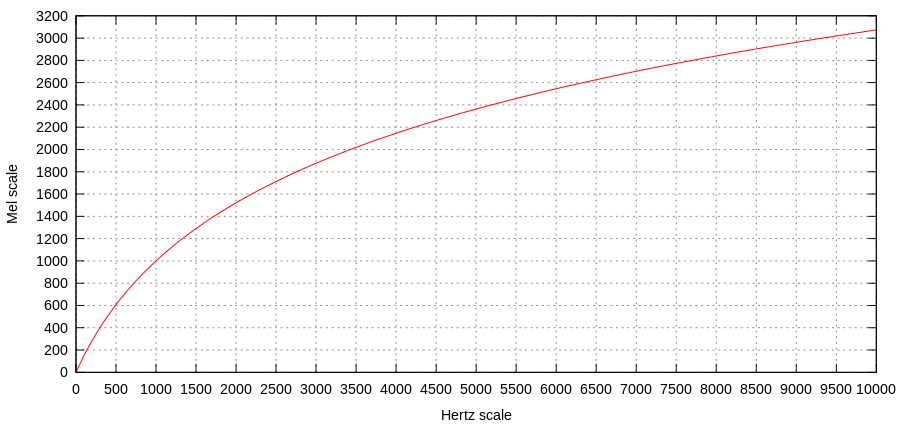
\includegraphics[width=0.8\linewidth]{Chapitre1/figures/Mel-Hz_plot.svg.png}
   \end{center}
   \caption
   {Mel scale vs Hertz scale.}
   \label{fig:melvshertz}
\end{figure}


The Mel filter-bank magnitude response denoted as \textbf{F} $ \in \mathbb{R} ^{B \times M}$, is made up of coefficients for B triangular band-pass filters that have central frequencies that are evenly spaced on the Mel scale. This results in filters that are closely spaced at lower frequencies and widely spaced at higher frequencies. The coefficients of the triangular filters are chosen from the range [0, 1] and are scaled so that the area under each triangle for the magnitude response is roughly the same across the Mel bands. A visualization of the Mel filter-bank magnitude response can be found in Figure \ref{fig:melfilterbanks}.

\begin{figure}[htbp]
   \begin{center}
      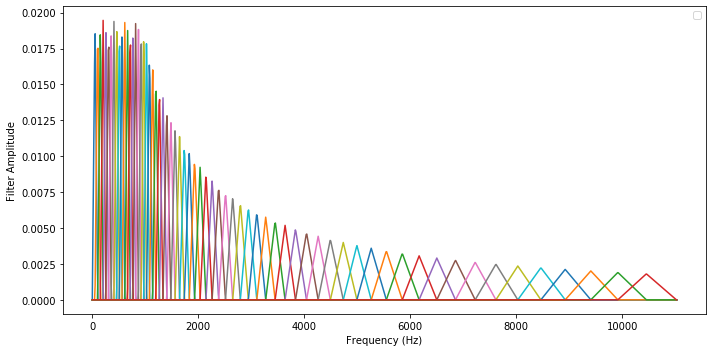
\includegraphics[width=0.8\linewidth]{Chapitre1/figures/triangular.png}
   \end{center}
   \caption{ Triangular Mel filter banks.}
   \label{fig:melfilterbanks}
\end{figure}


\subsubsection{Mel Spectrogram}

 Mel spectrograms are matrices that contain Mel band energy feature vectors for consecutive time frames generated by applying a Mel filter bank to the magnitude spectrogram at each time frame. The Mel filter bank uses the Mel scale and consists of triangular filters whose bandwidths increase with the central frequency of the filters. This results in higher frequency resolution in the lower frequency range and lower resolution in the higher frequency range. Log Mel spectrograms, which are created by taking the logarithm of Mel spectrograms, are a popular representation for tasks related to sound  classification and have been used in many  methods for environmental sound, rare sounds, sound events, and acoustic scenes \cite{DCASE2020Workshop, DCASE2019Workshop, DCASE2022Workshop, dcase2022, DCASE2021Challenge}. The number of Mel filter banks used in ESC is typically between 30 and 80, which is often smaller than the number of frequency bins used in the Short-Time Fourier Transform (STFT). As a result, Mel spectrograms provide a more compact representation than magnitude spectrograms. Several sound representations are illustrated in Figure \ref{fig:melspectrograms}.

\begin{figure}[htbp]
   \begin{center}
      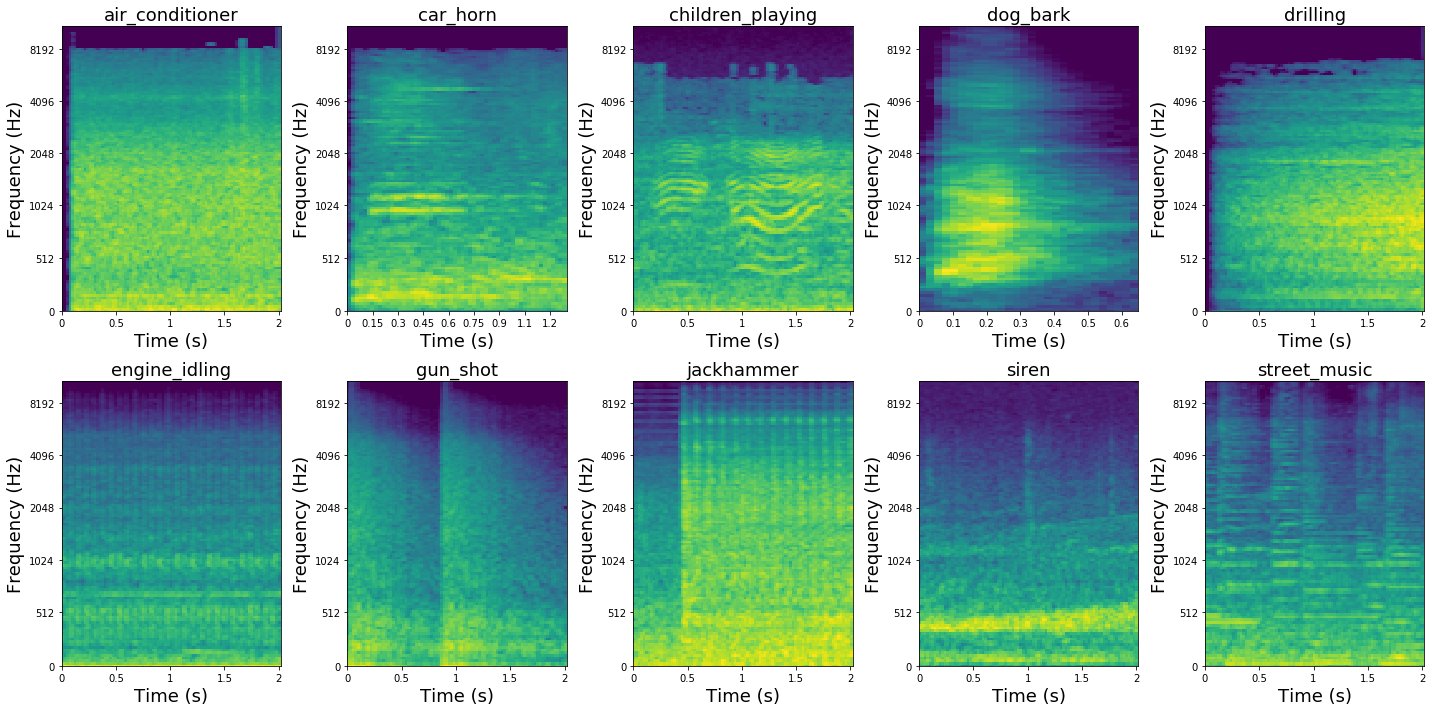
\includegraphics[width=1\linewidth]{Chapitre1/figures/Melspecs.png}
   \end{center}
   \caption
   {Log Mel spectrograms of different environmental sounds.}
   \label{fig:melspectrograms}
\end{figure}



\subsection{Mel-frequency cepstral coefficients (MFCC)}
% ----------------------------------------------

MFCCs, which stand for Mel-frequency cepstral coefficients, are a popular method of representing speech and audio data in processing applications. This method involves converting the Mel spectrogram into a log Mel spectrogram by taking the logarithm and then using the DCT (Discrete Cosine Transform) to calculate cepstral coefficients from the Mel-scaled log-power spectrum. DCT is used to decorrelate the features in the adjacent windows obtained in the log Mel spectrogram, as visualized in Figure \ref{fig:MFCCS}.  MFCCs are widely used in speech recognition, speaker identification, and music classification tasks.

\begin{figure}[htbp]
   \begin{center}
      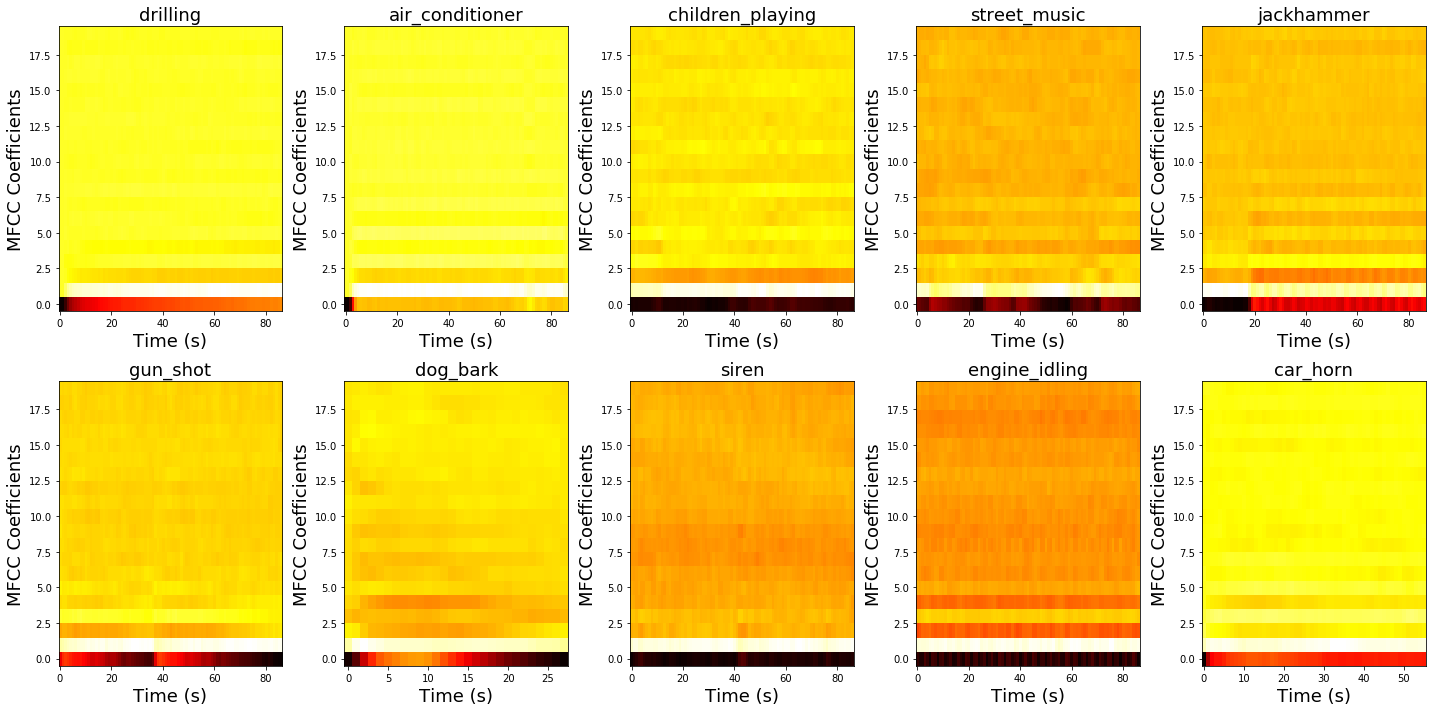
\includegraphics[width=1\linewidth]{Chapitre1/figures/MFCCSs.png}
   \end{center}
   \caption { Mel frequency cepstral coefficients of different environmental sounds.}
   \label{fig:MFCCS}
\end{figure}


% ---------------------------------------------


\subsection{Other feature extraction methods} 
There are several methods for representing sounds that use a magnitude spectrogram as the base, a visual representation of the frequency content of a sound over time. One such method is the Gamma-tone spectrogram \cite{patterson1992complex, slaney1993efficient}, which has also been used for machine hearing and has been proposed for detecting rare sound events \cite{plinge2014bag, yang2018sound, phan2017dnn}. It is based on the equivalent regular bandwidth scale and is used to extract acoustic features related to human auditory perception. Another method is the Spectrogram Image Feature (SIF), which involves converting the magnitude spectrogram into an RGB image based on the normalized amplitudes of the spectrogram \cite{5672395}.  This method has been suggested for sound event classification \cite{6338274}. The histogram of oriented gradients (HOG) is another image processing-based feature extraction method that uses the change in intensity (amplitude) in the spectrogram to classify acoustic scenes and events\cite{lim2015robust}. 

In addition to spectrogram-based features, another signal-to-feature transformation is the wavelet transform. The wavelet transform is a windowed Fourier transform in the time domain. Wavelet analysis provides the solution for analyzing non-stationary data \cite{ricker1940form} overcome limitations of STFT because the window is scaled in both time and frequency \cite{wirsing2020time}. 


\section{Machine Learning for Environmental sound classification} 
\label{chapter:backroundMachineLearningESC}
Machine learning is a part of artificial intelligence that deals with the development of algorithms or models that can learn from data and make predictions on new data. In machine learning, a computer is trained on a dataset and makes predictions or decisions without being explicitly programmed to perform the task. The goal of machine learning is to build models that can be generalized to new, unseen data, rather than just memorizing the patterns in the training data.

Machine learning methods have been widely used for the detection of sound events, which are described by the discrete occurrence of specific noise or sound patterns in an audio signal. These methods are comprised of training a model on a large dataset of audio examples, annotated by humans or machines, where the specific sound event has been identified or labeled. Once the model is trained, it is tested with an unseen audio example to detect and classify the sound automatically. Machine learning approaches can be highly effective for sound event detection, as they can learn complex patterns and relationships in the data that may be difficult to capture using traditional, rule-based methods. There are a variety of machine learning algorithms that have been applied to sound event detection, including Support Vector Machines (SVM), random forests, and deep neural networks.

A formal definition for machine learning algorithm is provided by \cite{mitchell1997machine}: 

\boitemagique{Machine Learning}{"A computer program is said to learn from experience E with respect to some class of tasks T and performance measure P, if its performance at tasks in T, as measured by P, improves with experience E". }


In this thesis, the task $T$ is globally defined as an environmental sound classification in this thesis. For environmental sound classification, the experience, $E$, is often represented by the acoustic features accompanied by the labels of the audio recordings in the database.  The acoustic features can be represented by an input matrix, $X$, which comprises of $M$ acoustic features extracted from each frame of the audio recording divided into $T$ time frames. The labels are encoded, generally one hot encoding, as a binary target output matrix $Y$, with $C$ referring to the total number of classes of sound events. The target output labels are the annotations of the target sound input. If a particular sound event $p$ is present in an audio recording then $Y_p$ is set to $1$, otherwise, it is set to $0$. The reference labels are used in the machine learning model for classification. Then the performance of this model is evaluated using metrics such as accuracy and error rate discussed in the upcoming section. 


The objective of the machine learning task is to develop a function $F$ that can accurately map input data $X$ to target output $Y$. In sound classification, the input is represented by $X$, the acoustic feature, and the output target is the label or the target output matrix $Y$. The function $F$ takes an acoustic feature matrix and produces a probability vector $\hat{Y}$ indicating the likelihood of the sound event being present in that input. During the learning phase, the parameters of this function are adjusted to minimize the difference between the predicted output $\hat{Y}$ and the actual target output $Y$. 
In the usage phase, when the target output is either not available or being used for evaluation purposes, the predicted output $\hat{Y}$ is used to identify the most likely sound event label in a given input. In the case of ESC, this is the sound event label with the highest probability as shown in Figure \ref{fig:Machinelearning}.


\begin{figure}[htbp]
   \begin{center}
      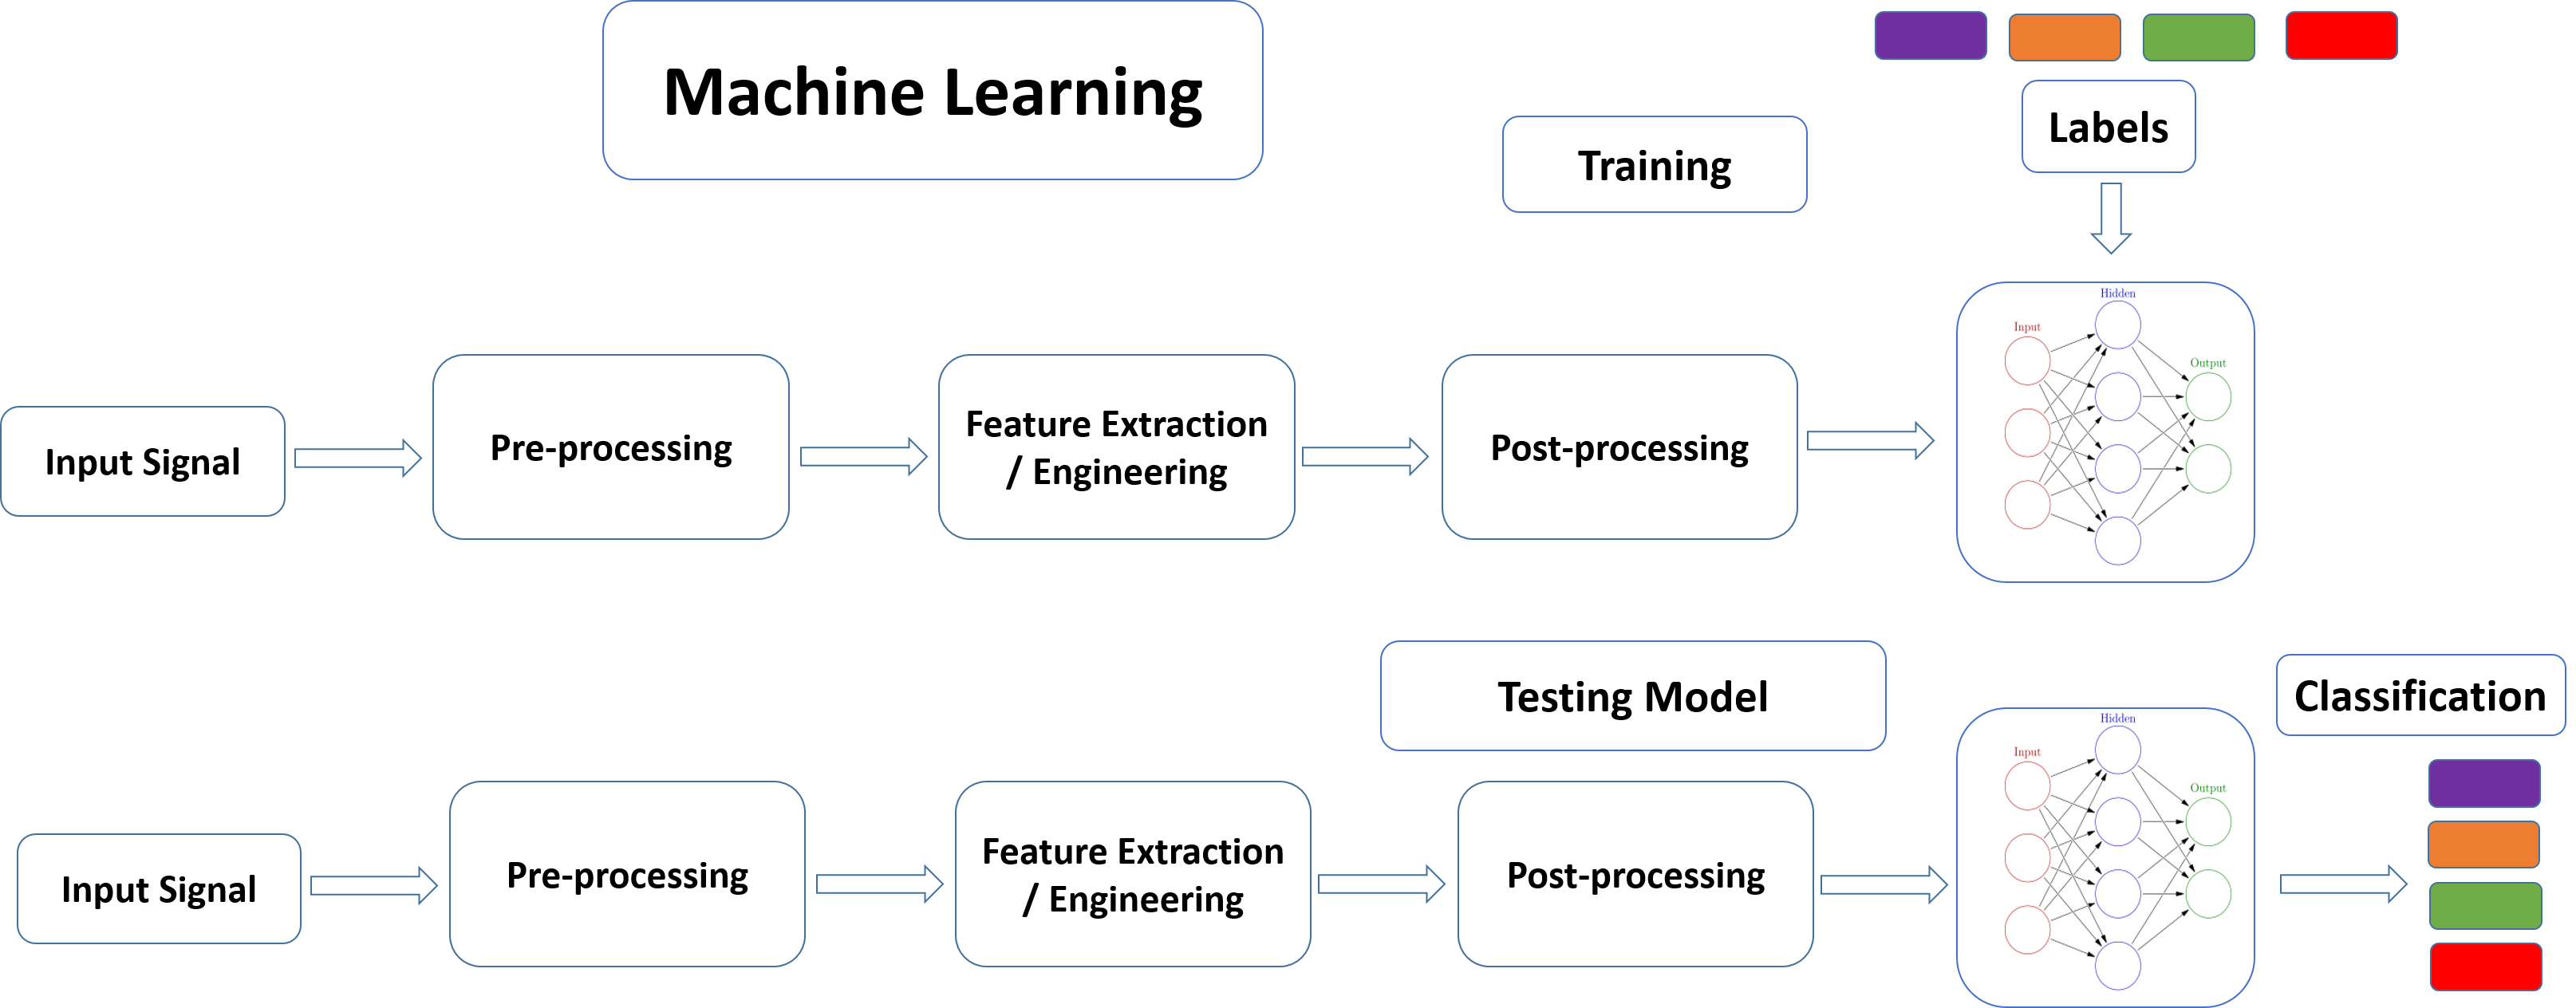
\includegraphics[width=1\linewidth]{Chapitre1/figures/Machinelearning2.png}
   \end{center}
   \caption{ Block diagram of machine learning method with neural networks.}
   \label{fig:Machinelearning}
\end{figure}

\section{Artificial Neural Networks} 

An artificial neural network (ANN) is a type of machine learning algorithm that is inspired by the structure and function of the human brain  as depicted in Figure \ref{fig:neuron} \cite{karpathy2015neural}. The human brain is composed of billions of interconnected neurons, which are stimulated by various electrochemical signals in order to process and transmit information. ANNs attempt to replicate the structure and function of a biological neural network, but use a simplified set of concepts from biological neural systems. ANNs are specifically designed to simulate the electrical activity of the brain and nervous system and are composed of processing elements (also known as neurons or perceptrons) that are connected to each other in a way that emulates the connections between neurons in the brain. The processing elements in an ANN receive input data, perform a computation on the data, and transmit the output data to other processing elements or external destinations.


\begin{figure}[htbp]
   \begin{center}
      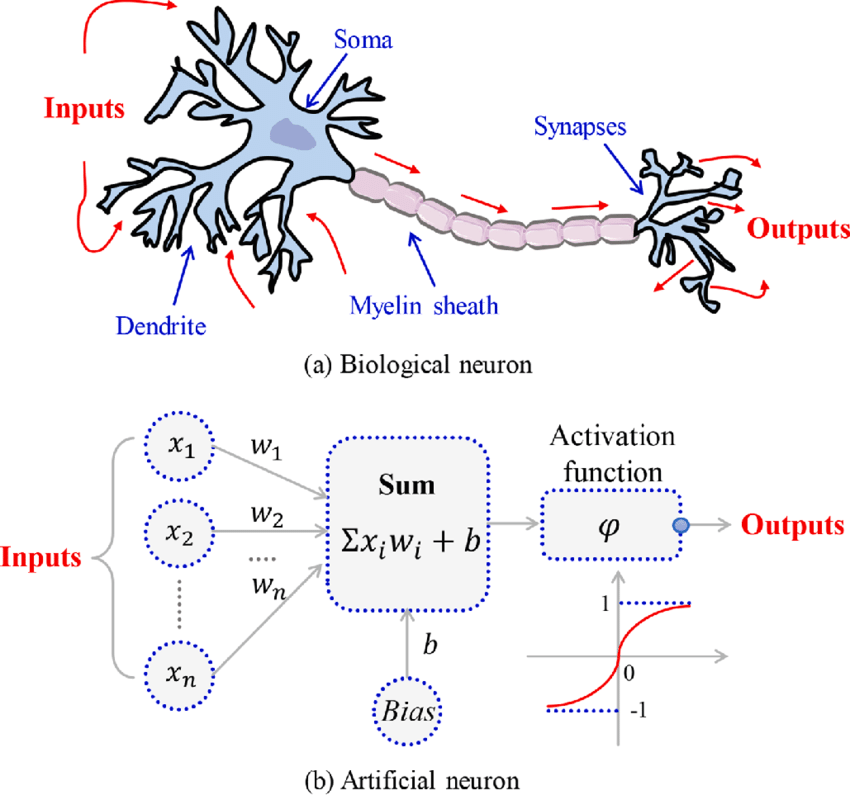
\includegraphics[width=0.6\linewidth]{Chapitre1/figures/neuronsnew.png}
   \end{center}
   \caption { Biological neuron and artificial neuron.}
   \label{fig:neuron}
\end{figure}


Different types of signals, such as sensory, audio, and visual signals, can stimulate different paths of neurons in the brain, and the signal information is processed through a collective set of neuron stimulations. From the moment of birth, the neurons in the brain specialize in processing certain types of signals and continuously improve their ability to create a mapping between the input signal and its cognitive representation. For example, when we hear human speech, a special kind of audio signal used for communication, it is first transformed into electrochemical signals in the ear and brain. The cochlea is a spiral-shaped structure in the ear that is responsible for converting sound waves into electrical signals. These signals are then processed by the neurons in the brain through a series of stimulations, which map the signals to a set of phonemes, or units of sound, which have a shared cognitive representation for human communication.

ANNs attempt to replicate this process of information processing and mapping by using a set of interconnected processing elements, which receive input data and transmit output data based on the weights of their connections and the activation functions applied to the input data. 
Each neuron has certain parameters, such as weights and biases, which are adjusted iteratively through a process such as a gradient optimization in order to minimize an error function between the desired output and the estimated output. The layer that receives the input signal is called the input layer, the layer that determines the final output of the network is called the output layer, and the layers in between are called hidden layers. ANNs have a set of hyper-parameters that determine the network architecture, such as the number of hidden units and layers, and the training procedure, such as the optimization method and regularization parameters. ANNs with multiple hidden layers are often referred to as deep learning or deep neural networks (DNNs). In this context, "deep learning" refers to all ANN methods that utilize multiple hidden layers. Deep learning has become increasingly popular in the field of machine learning due to the availability of large datasets, advanced training techniques, and increased computational power by GPUs.


\subsection{Feed-forward Neural Networks} 
Feed-forward neural networks (FNN) are a type of artificial neural network that processes input data and generates output data in a single direction, without looping back. These networks, also known as fully connected networks or multi-layer perceptrons (MLPs), consist of layers of interconnected artificial neurons, or processing elements, that receive input data, apply computation based on the weights of their connections and activation functions and transmit output data to the next layer.

 Each neuron in a feed-forward network receives input from multiple other neurons in the previous layer, performs a computation on the input data, and transmits the output to multiple neurons in the next layer. The input layer receives the raw input data, and the output layer generates the final output of the network. The layers in between the input and output layers are called hidden layers, and their purpose is to extract features and patterns from the input data that can be used to make predictions or classifications.

 The calculation of FNN is calculated in two stages, first, the weighted sum \textbf{z} of the output of the previous connected layer of neurons is calculated and an additional bias \textbf{b} is added, and represented as:

\begin{equation}
z_{j}^{(l)}=\sum_{1\leq k\leq n^{(l-1)}}w_{j,k}^{(l)}h_{k}^{(l-1)}+b_{j}^{(l)}
\label{eq:wb}
\end{equation}

where \textbf{$W_{j}^{(l)}=(w_{j,k}^{(l)})_{1\leq k\leq n^{(l-1)}}$} represents the input weights in the neuron j from the layers \textit{l,} $n^{(l-1)}$ is the number of outputs of the layer $(l-1)$, $h_{k}^{(l-1)}$ is the output for the neuron \textit{k} in the layer \textit{l-1}, $z_{j}^{(l)}$ is the weighted sum for the neuron \textit{j} in $l^{th}$ layer.

Secondly, a non-linear function is applied to the output of the neuron $k$ in the layer $l-1$, to map the non-linear relationship in the input. In a neural network, non-linear functions are used to introduce non-linearity into the model. This is important because many real-world problems are non-linear in nature, and a model that is only capable of learning linear relationships will not be able to accurately capture the complexity of these problems. The non-linearity function is defined as $\sigma$ and the relation is defined as:


\begin{equation}
h_{k}^{l}=\sigma{(z_{k}^{(l)})}
\label{eq:wb2-1}
\end{equation}

The non-linearity function is most commonly known as \textit{activation function}, and this activation function empowers the neural networks to approximate complex functions. Let $h^{(l-1)}\in\mathbb{R}^{n^{(l-1)}}$ be input to the~ $l^{th}$  layer (outputs of the $(l-1)^{th}$layer), and $h^{(l)}\in\mathbb{R}^{n^{(l)}}$ is its output, then the output of the neuron $k$ in the layer $l$ is defined as :

\begin{equation}
h_{k}^{(l)}=\sigma{(W_{k}^{(l)}\left(h^{(l-1)}\right)^{T}+b_{k}^{(l)})}\label{eq:wb3}
\end{equation}

and $h^{(l)}\in\mathbb{R}^{n^{(l)}}$ is defined as: 

\[
h^{(l)}=\sigma{(\boldsymbol{W}^{(l)}\left(h^{(l-1)}\right)^{T}+b^{(l)})}
\]

where 
\[
\boldsymbol{W^{(l)}}=(w_{j,k}^{(l)})_{\begin{array}{c}
1\leq j\leq n^{(l)}\\
1\leq k\leq n^{(l-1)}
\end{array}}
\]
\[
\boldsymbol{b}=(b_{j}^{(l)})_{1\leq j\leq n^{(l)}}
\]
\

Non-linear functions that are frequently used include the logistic sigmoid function (\textit{sigm}), the hyperbolic tangent function (\textit{tanh}), and the rectified linear unit function (\textit{ReLU}). These functions are element-wise, meaning that they operate on individual elements in an array or matrix, and their equations are discussed in the following section. 

Feed-forward neural networks are characterized by the fact that information flows through the model in a single direction, from the input $\textbf{x\ensuremath{\mathbb{\in R}^{n}}}$ to the output $\mathbf{y}\in\mathbb{R}^{m}$, without any feedback connections. In these models, the output is determined by the intermediate computations used to define the function, \cite{Goodfellow-et-al-2016}:

\[
f:\begin{array}{ccc}
\mathbb{R^{\mathit{n}}} & \rightarrow & \mathbb{R^{\mathit{m}}}\\
\boldsymbol{x}=(x_{1},...,x_{n}) & \rightarrow & \boldsymbol{y}=(y_{1},...,y_{m})=f(x)
\end{array}
\]

The goal of a feed-forward network is  to find the appropriate parameters (weight and biases: $\boldsymbol{W}$ and \textbf{$\boldsymbol{b}$}) that result in the best function approximation. The weight $\boldsymbol{W}$ and biases \textbf{$\boldsymbol{b}$} are defined as:

\[
\boldsymbol{W}=(w_{j,k}^{(l)})_{\begin{array}{c}
1\leq j\leq n^{(l)}\\
1\leq k\leq n^{(l-1)}\\
1\leq l\leq L
\end{array}}
\]
\[
\boldsymbol{b}=(b_{j}^{(l)})_{\begin{array}{c}
1\leq j\leq n^{(l)}\\
1\leq l\leq L\\
\\
\end{array}}
\]
 

So the variables are the parameters, that we denote for simplification $\boldsymbol{\theta}=\boldsymbol{(W},\boldsymbol{b)}$ and the feed-forward network can be defined as :

\[
\widehat{f}:\begin{array}{ccc}
\mathbb{R^{\mathit{n+p}}} & \rightarrow & \mathbb{R^{\mathit{m}}}\\
(\boldsymbol{x},\boldsymbol{\theta}) & \rightarrow & \boldsymbol{y}=(y_{1},...,y_{m})=\widehat{f}(\boldsymbol{x},\boldsymbol{\theta})
\end{array}
\]


where, $n$ is the number of input and $p$ is \textit{parameters} and $\widehat{f}$ represent the neural network model. A feed-forward neural network is illustrated in Figure \ref{fig:DNN}. For the model shown in the figure, the model takes the input feature vector, in our case acoustic feature per time frame, as input and calculates the probability for each fourth output nodes, sound classes present in the acoustic feature in our case. If the target output vector y is binary-encoded (common in SED tasks), the weighted sum of each neuron in the output layer is passed through an activation function that bounds the output between 0 and 1, allowing the network output $\boldsymbol{\hat{y}}$ to be
interpreted as the estimated probabilities of the sound events being present in the frame.

Feedforward neural networks play a crucial role in the field of machine learning and are the foundation of many practical applications. For instance, \textit{convolutional neural networks}, which are used for object recognition from images, are a type of \textit{feed forward network}. Feedforward networks are a fundamental concept that leads to the development of recurrent neural networks, which are used in natural language processing applications.

When feed-forward networks are extended to include feedback connections, they become recurrent neural networks, which will be discussed in a later section.


\begin{figure}[htbp]
   \begin{center}
      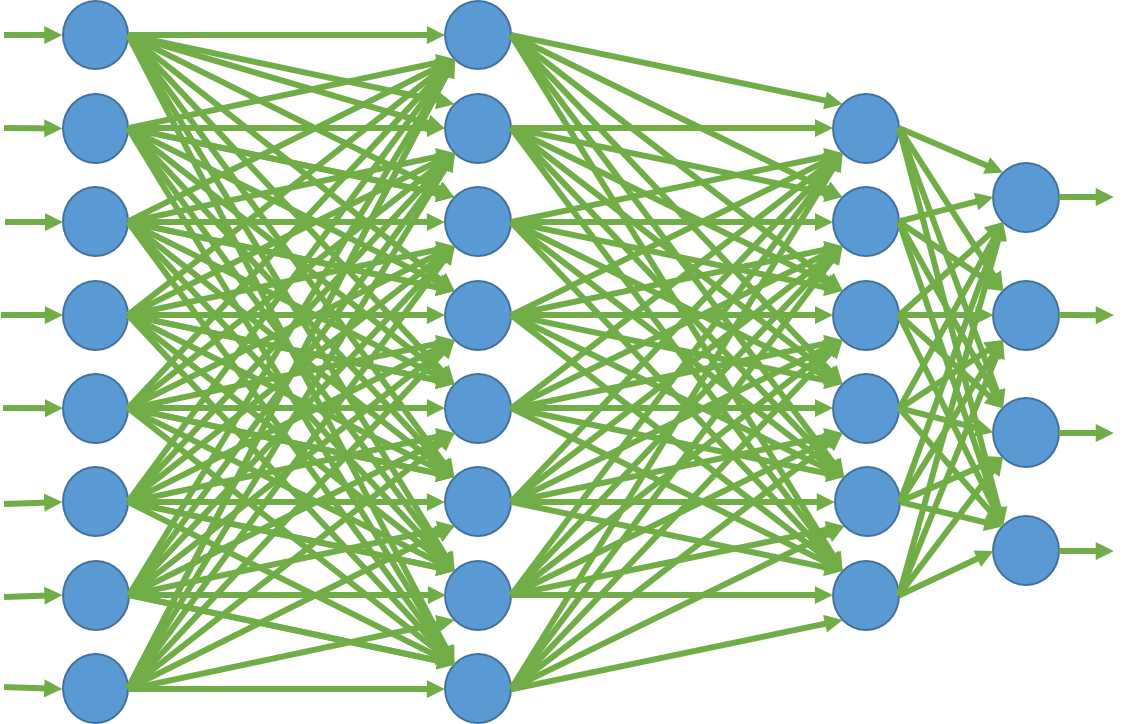
\includegraphics[width=0.8\linewidth]{Chapitre1/figures/DNN.png}
   \end{center}
   \caption{Feed forward neural network. First layer is the input layer, followed by two hidden layers and a output layer at the end.}
   \label{fig:DNN}
\end{figure}



\subsection{Recurrent Neural Networks}

Recurrent neural networks (RNN) are a type of artificial neural network that is specifically designed to handle sequential data. This quality has made RNNs popular in the tasks related to language translation, speech recognition, and natural language processing \cite{datta2020neural, sak2014long, makino2019recurrent, chernykh2017emotion, zhang2021attention, parascandolo2016recurrent, kerkeni2019automatic, kerkeni2019automatic2}. In a deep neural network, the input data is typically transformed into a fixed-length feature vector. This feature vector is passed and processed by the hidden layers before generating class estimation at the output layer. This means that at each time step, the prediction made by the \textbf{y} is only based on the input \textbf{x} at present and does not take into account any context from the previous input. This can be problematic for certain models where context is important. 
In contrast, RNN processes the input data element one at a time while keeping the states of elements passed before in the sequence by using hidden layers or hidden states. In RNN, the value of each hidden layer depends not only on the values of the layers below it at the current time step but also on the value of the same layer at the previous time step. 
The value of the hidden layer, represented by $h_t^{(l)}$ of the $l-th$ layer at time t, is given by:

\begin{equation}
    \label{eq:rnn}
    h_t^{(l)} = \sigma (U^{(l)} h_{t-1}^{(l)} + W^{(l)}h_{t}^{(l-1)} + b^{(l)})
\end{equation}

Here, $U^{(l)}$ matrix is the \textit{recurrent weight matrix}. At each time step, the RNN cell processes the current input and the previous hidden state, producing a new output and updating the hidden state with the new information as shown in Figure \ref{fig:rnn} \cite{colah_2015}. This process is repeated for each element in the sequence, allowing the RNN to build up a representation of the entire sequence over time.


RNNS processes an input sequence in a single direction, using information from past contexts to calculate the output for the current time step. In some cases, it may be beneficial to also process the input sequence in the opposite direction in the future context. In this case, $\textit{bidirectional RNN}$ have been proposed \cite{schuster1997bidirectional}. In addition to the forward chain in the hidden layer in RNN, a backward chain is also included. Both chains of the hidden layer are connected to the  forward and backward chains in the next hidden layer. Let $\overrightarrow{h_t^{(l)}}$ represent the output of the $l-th$ layer in forward direction, $\overleftarrow{h_t^{(l)}}$ represent the output of the $l^{th}$ layer in backward direction and $h_{t}^{(l)}$ represents the concatenation of the two. The relation is described by :

\begin{equation}
    \label{eq:BiRNN1}
    \overrightarrow{h_t^{(l)}}  = \sigma (\overrightarrow{U}^{(l)} \overrightarrow{h}_{t-1}^{(l)} + W^{(l)}h_{t}^{(l-1)} + \overrightarrow{b}^{(l)})
\end{equation}
\begin{equation}
    \label{eq:BiRNN2}
        \overleftarrow{h_t^{(l)}}  = \sigma (\overleftarrow{U}^{(l)} \overleftarrow{h}_{t-1}^{(l)} + W^{(l)}h_{t}^{(l-1)} + \overleftarrow{b}^{(l)})
\end{equation}


Here, $\overrightarrow{U}^{(l)}$ and $\overrightarrow{b}^{(l)}$ are the forward recurrent weights and biases. Similarly, $\overleftarrow{V}^{(l)}$ and $\overleftarrow{b}^{(l)}$ are the weights and biases in the backward direction. A bidirectional RNN has access to the entire input sequence when making a prediction at any time step, providing it with unlimited context. 


\begin{figure}[htbp]
   \begin{center}
      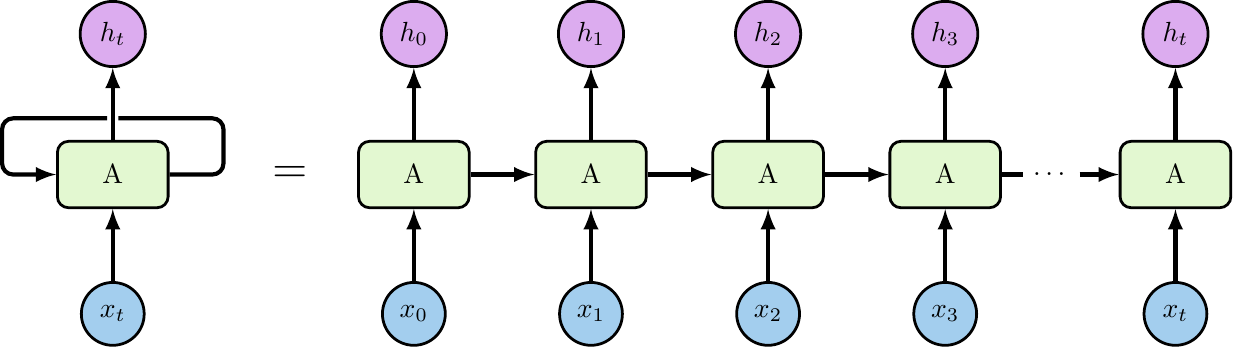
\includegraphics[]{Chapitre1/figures/rnn.png}
   \end{center}
   \caption{ Recurrent Units in Recurrent neural networks.}
   \label{fig:rnn}
\end{figure}



 RNNs face difficulty in modeling long-term dependencies, as the impact of past time steps on the current output tends to decrease exponentially over time due to the $\textit{gradients vanishing}$ problem. This limits the ability of RNNs to effectively incorporate long temporal context, despite their theoretical potential to do so \cite{hochreiter2001gradient}. 

 To address the issues with traditional RNNs, gated recurrent layer methods such as g$\textit{ated recurrent units}$ (GRUs) and $\textit{long short-term memory networks}$ (LSTMs) were introduced. These methods use units called cells, which combine multiple gate activations to produce their output. LSTMs have external input, forget, and output gates, while GRUs have an update and reset gates. These gates, which are made up of weights and an activation function, allow the cells to accumulate and selectively preserve information from past time steps in a cell state. During training, the gate weights learn how to combine the cell state and the input for the current time step to produce the gated unit output for the current time step. 

 The cell structure of LSTM and GRU are shown in figure \ref{fig:lstm} and \ref{fig:GRU} respectively \cite{colah_2015}. The three types of gates in an LSTM network are the input gate, forget gate, and output gate. These gates use the following equations to determine how to update the state of the network at each time step:


\begin{align}
 i_t &= \sigma(W_i \cdot x_t + U_i \cdot h_{t-1} + b_i) \\
 f_t &= \sigma(W_f \cdot x_t + U_f \cdot h_{t-1} + b_f) \\
 o_t &= \sigma(W_o \cdot x_t + U_o \cdot h_{t-1} + b_o) \\
 c_t &= f_t \cdot c_{t-1} + i_t \cdot \tanh(W_c \cdot x_t + U_c \cdot h_{t-1} + b_c) \\
 h_t &= o_t \cdot \tanh(c_t)
\end{align}

where,

\begin{itemize}[label=$\cdot$]
    \item $x_t$ is the input at time step $t$
    \item $h_{t-1}$ is the hidden state at time step $t-1$
    \item $i_t$, $f_t$, $o_t$ are the input, forget, and output gates, respectively, at time step $t$
    \item $W$, $U$, and $b$ are learn-able weight matrices and biases
    \item $c_t$ is the cell state at time step $t$
    \item $c_{t-1}$ is the cell state at time step $t-1$
    \item $h_t$ is the hidden state at time step $t$
    \item $\sigma$ is the logistic sigmoid function 
\end{itemize}

\begin{figure}
  \subfigure[Long short term memory cell]{
    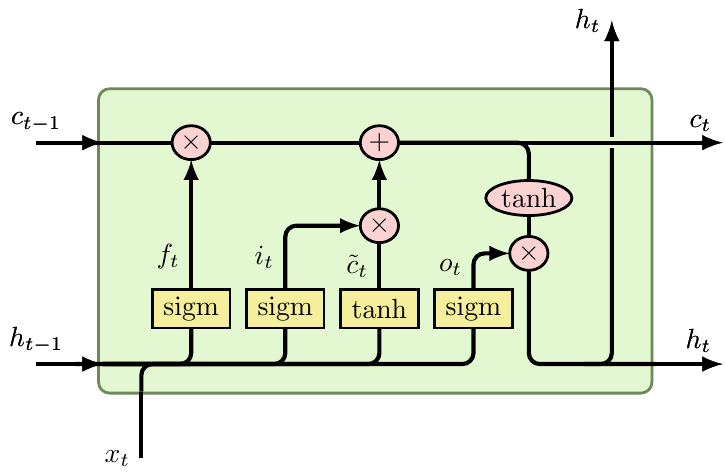
\includegraphics[width=0.45\linewidth]{Chapitre1/figures/lstmcell.png}
    \label{fig:lstm}
  }
  \subfigure[Gated Recurrent unit cell]{
    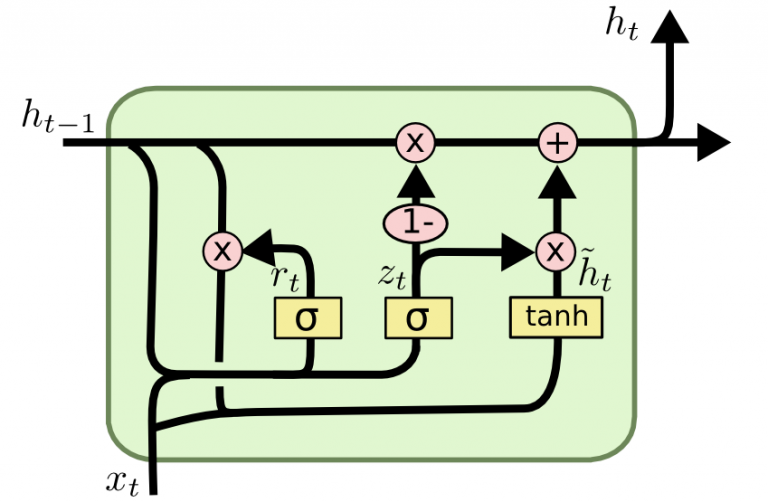
\includegraphics[width=0.45\linewidth]{Chapitre1/figures/GRU-768x502.png}
    \label{fig:GRU}
  }
  \caption{LSTM and GRU Cell.}
  \label{fig:LSTM_GRU}
\end{figure}

Both LSTMs and GRUs are able to capture long-term dependencies in data, however, they differ in a few aspects as shown in Fig.\ref{fig:LSTM_GRU}. LSTMs have three types of gates (input, forget, and output gates) while GRUs have only two (reset and update gates). LSTMs have a separate cell state that is updated using the input, forget, and output gates, while GRUs do not have a separate cell state and update their hidden state directly using the reset and update gates. LSTMs have more parameters than GRUs, which can make them more difficult to train and may require more computational resources. In general, LSTMs and GRUs perform similarly on many tasks, but LSTMs may be more suitable for tasks that require long-term dependencies to be captured over longer sequences, while GRUs may be more suitable for tasks that require the model to learn more quickly.

\subsection{Convolutional Neural Networks}

Convolutional neural networks (CNNs) are a type of deep neural network that performs relatively well for image classification and recognition tasks. They are able to learn the important features and objects in an image by assigning weights and biases to different aspects of the input data. The design and architecture of CNNs are inspired by the structure of the visual cortex in human and animal brains. Each neuron is responsible for processing a specific region of input data, known as \textit{receptive field} that is sensitive to the specific patterns  in the visual environments. The receptive field of multiple neurons overlaps to cover the entire input data.

The fundamental component of CNN is a \textit{convolutional layer} inter-weaved with \textit{pooling layers}, which are responsible for extracting features from the input data. The convolutional layer contains a collection of filters, also called kernels or weights, which are scanned over the input data and detect specific patterns. Each filter is a small matrix of weights that is applied to a small region of the input data.
The output of this process is a \textit{feature map}, which is the representation of the responses of the filters at each location in the input data. 

In a multi-layer convolutional network, the output of one layer serves as the input for the next layer. This output typically consists of the results of multiple convolutions at each position. When working with images, we typically represent the input and output of the convolutional operation as 3-dimensional tensors, with indices for the different channels and the spatial coordinates within each channel. In practice, software implementations of convolutional networks often use batch processing, which involves 4-dimensional tensors with an additional index for the different examples in the batch. For simplicity, we will describe the operations here without considering the batch axis.



The convolution operation between a filter $\textbf{F}$ and an input image $\textbf{X}$ with height $h$, width $w$, and number of channels $c$ can be represented mathematically as:

\begin{equation}
    \label{eq:Conv1}
    H_{i,j,k} = \sigma\left( \sum_{c=1}^{C} \sum_{m=1}^{S} \sum_{n=1}^{S} X_{s\cdot i + m, s\cdot j + n, c} \cdot F_{m,n,c,k} + B_k \right)
\end{equation}

Where $H_{i,j,k}$ is the activation at position $(i,j)$ in the output feature map for channel $k$, $C$ is the number of channels in the input image, $S$ is the size of the filter, $s$ is the stride, $B_k$ is the bias for channel $k$, and $F_{m,n,c,k}$ is the entry of the filter $F$ at position $(m,n)$ for channel $c$ and channel $k$. The double summation over $m$ and $n$ is taken over the height and width of the filter, while the summation over $c$ is taken over the number of channels in the input image. The $i$ and $j$ indices indicate the position of the filter in the input image.

The final output feature map has shape $(h', w', k)$, where $h'$ and $w'$ are the height and width of the output feature map, and $k$ is the number of channels in the output feature map. Where $\sigma$ is the activation function. The kernel slides over the input to extract the local representation and is generally smaller in size as compared to the input as visualized in Figure \ref{fig:Convolution}.



\begin{figure}[htbp]
   \begin{center}
      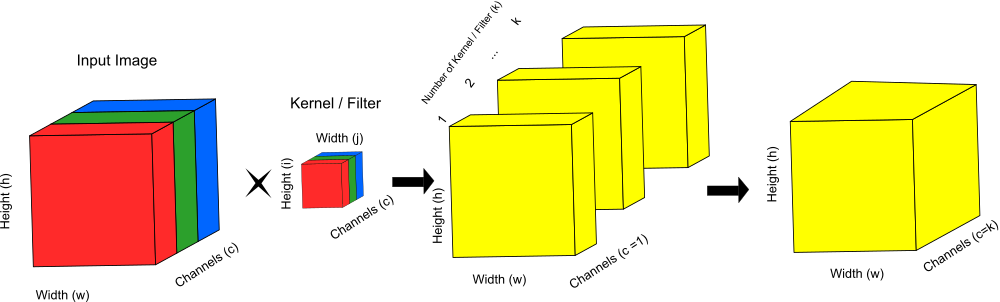
\includegraphics[width=1\linewidth]{Chapitre1/figures/Convolution.png}
   \end{center}
   \caption{ Convolution operation in convolutional neural networks (CNN)}
   \label{fig:Convolution}
\end{figure}



A pooling layer operates by dividing the input feature map into non-overlapping regions, each containing $m \times n$ pixels. The stride of the pooling layer is equal to $m \times n$. For each region, the pooling layer computes a statistic, which can be either the maximum or the average value. These are the most commonly used statistics in pooling layers.

When applied to image recognition tasks, a neural network typically makes a prediction for an entire image represented as 1 or 3 input feature maps (for gray-scale or color images, respectively). The layers of the network are usually arranged in a way that involves increasing the number of feature maps through the use of convolutional layers and decreasing the size of the feature maps through the use of pooling layers. Once the feature maps become small enough, they are often flattened into a single vector and processed by fully connected layers to make the final prediction.

The
Convolutional layers are applied to the feature image, time-frequency representation for sound, along with pooling layers. The image is transformed into a sequence by subsequent application of convolutional and pooling layers as shown in Figure \ref{fig:CNN}. This sequence is used as input to fully-connected neural networks. In contrast to fully-connected neural networks, where each input feature is connected to a hidden unit in the next layer, convolutional layers use shared parameters among the input features and train the kernel parameters to learn local patterns that can be found anywhere in the input. This is particularly useful for ESC, where a sound event should be detected from a spectrogram regardless of its position in time. Additionally, convolutional layers, which typically consist of tens or hundreds of kernels, are often more memory-efficient than fully-connected neural networks due to the reduced number of weights. Convolutional layers in ANNs are typically used to identify important features. These features are then introduced into another layer in the ANN. If this input needs to be in the form of a vector, such as for use in an RNN, the features from each feature map are combined along the frequency axis to form a single vector for each time step. 

CNNs have several advantages, including shift in-variance and locality. Shift in-variance means that the prediction for an image should not change if the object of interest moves within the image. This property is also desirable for audio signals, as a phoneme or sound event should be recognized regardless of its position in the audio signal, and a limited shift along the frequency axis should not affect the prediction. CNNs achieve shift in-variance by applying the same convolution kernel to all parts of the input. Locality means that the network has a sense of which parts of the input are close to each other and which parts are far apart. This is achieved through the use of neurons that only receive information from neurons representing a neighboring region in the lower layer. As a result of locality, CNNs do not have the unlimited context that RNNs do when applied to audio. However, tasks involving audio may not require unlimited context, as audio usually does not exhibit long-range dependence in the same way that natural language does.


\begin{figure}[htbp]
   \begin{center}
      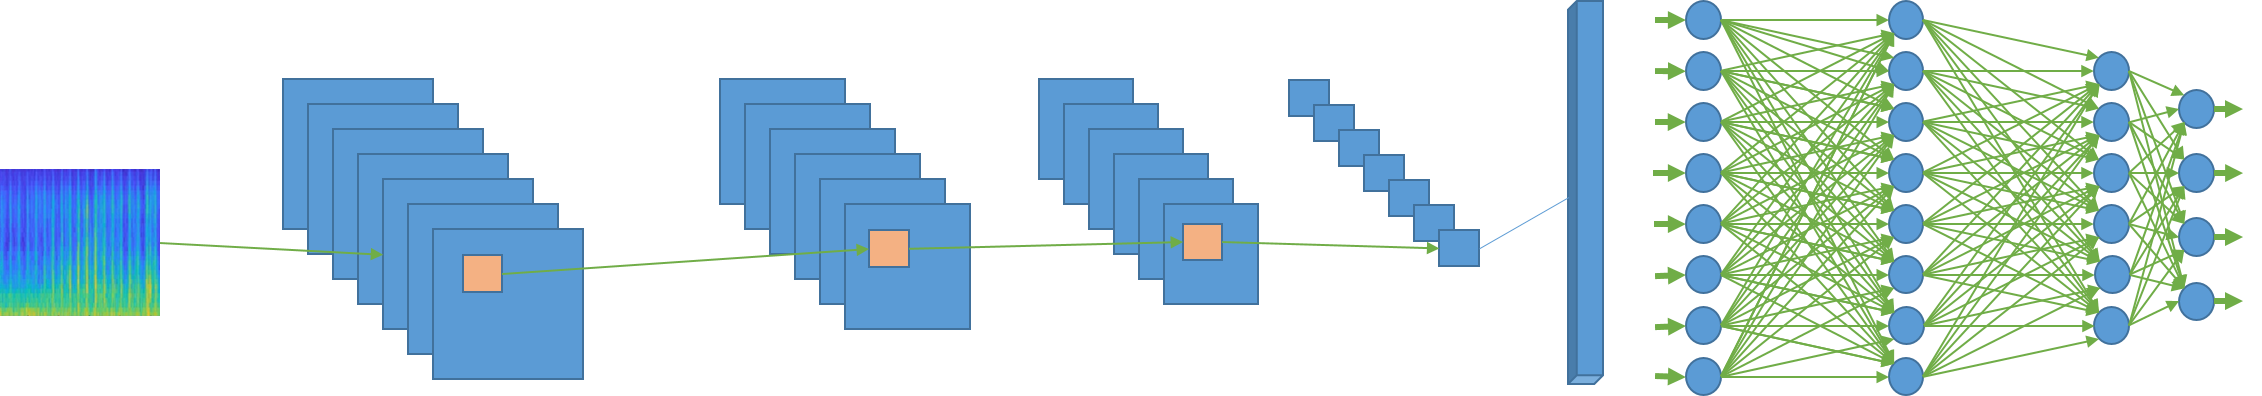
\includegraphics[width=1\linewidth]{Chapitre1/figures/CNN.png}
   \end{center}
   \caption { Convolutional neural network (CNN) on a spectrogram.}
   \label{fig:CNN}
\end{figure}

\vspace{-2em} % reduce vertical space between text and image

\subsection{Depthwise separable convolution networks }

 A depthwise separable convolutional network (DS-CNN) is a type of CNN architecture that aims to reduce the number of parameters and computation required by a traditional CNN. This is achieved by breaking a standard convolutional layer into two separate layers: a depthwise convolution layer and a pointwise convolution layer \cite{chollet2017xception}.

The depthwise convolution layer applies a single filter to each input channel, rather than applying the same filter across all channels as in a traditional CNN. This results in a set of feature maps, one for each input channel. Let the input image tensor be denoted as $\mathbf{X}$ with dimensions $(h, w, c)$ where $h$ is the height, $w$ is the width, and $c$ is the number of channels. The first step of the DSCNN operation is the depthwise convolution operation, which is defined as follows:


\begin{equation}
\mathbf{Z}_{i,j,k} = \sum_{m=0}^{k-1} \sum_{n=0}^{f_{h}-1} \sum_{p=0}^{f_{w}-1} \mathbf{X}_{i-n,j-p,m} \cdot \mathbf{F}_{n,p,m,k}
\end{equation}


Where $\mathbf{Z}$ is the intermediate feature map with dimensions $(h, w, c)$, $\mathbf{F}$ is the depthwise filter with dimensions $(f_h, f_w, c, 1)$, $i$ and $j$ are the indices for the height and width respectively, $k$ is the channel index, and $m$, $n$, and $p$ are the indices for the filter height, width, and channel, respectively. As shown in Figure \ref{fig:Depthwise}.

\begin{figure}[htbp]
   \begin{center}
      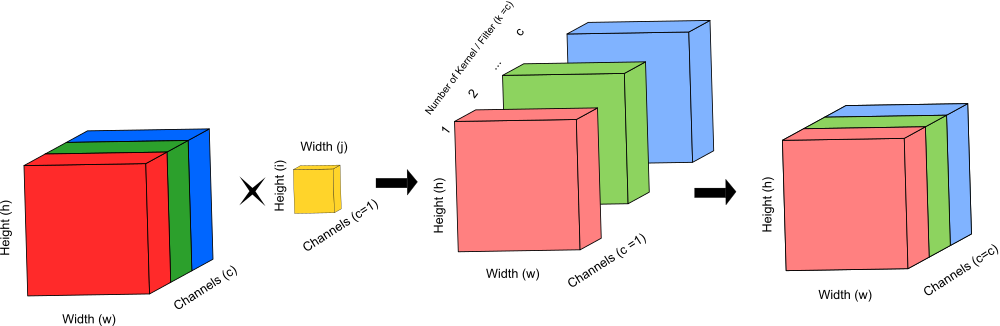
\includegraphics[width=1\linewidth]{Chapitre1/figures/Depthwise.png}
   \end{center}
   \caption{ Depthwise convolution operation on an input image.}
   \label{fig:Depthwise}
\end{figure}


The pointwise convolution layer then applies a 1x1 convolution to the set of feature maps output by the depthwise convolution layer. This combines the information across all channels and produces a single output feature map, which is defined as follows::

\begin{equation}
\mathbf{Y}_{i,j,k} = \sum_{m=0}^{c-1} \mathbf{Z}_{i,j,m} \cdot \mathbf{G}_{m,k}
\end{equation}

Where $\mathbf{Y}$ is the output feature map with dimensions $(h, w, k)$, $\mathbf{G}$ is the pointwise filter with dimensions $(c, k)$, and $k$ is the index for the number of output channels, depicted in Figure \ref{fig:Separable}.


\begin{figure}[htbp]
   \begin{center}
      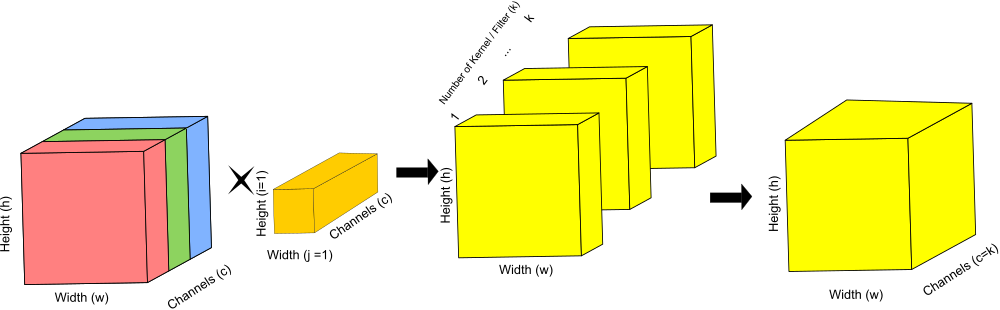
\includegraphics[width=1\linewidth]{Chapitre1/figures/Separable.png}
   \end{center}
   \caption{ Pointwise convolution operation on an input image.}
   \label{fig:Separable}
\end{figure}


The use of depthwise separable convolutions can greatly reduce the number of parameters in a CNN, as the number of parameters in the depthwise layer is equal to the number of input channels, while the number of parameters in the pointwise layer is equal to the number of input channels times the number of output channels. This can lead to faster training and better performance on some tasks.







\section{Neural network model training and evaluation} 
\subsection{Training of Model}
Training of a neural network model involves the adjustment of the model's weights and biases to minimize the error between the predicted output and the true output based on the dataset presented. This is typically done using an optimization algorithm, such as stochastic gradient descent (SGD), which adjusts the weights and biases iteratively to minimize the loss function. The loss function is a measure of the difference between the predicted output and the true output, and the optimization algorithm attempts to find the best combination of weights and biases that minimizes this difference.

The parameters of the neural network $\theta$ are typically initialized with small, randomly generated values drawn from a normal distribution. The input data is then passed through the network, and the output of the network is calculated $ \hat{y} = f(x, \theta)$. This process is known as forward pass or forward propagation. To evaluate how close the predicted output $\hat{y}$ is to the true output $y$, we calculate the loss $l(y,\hat{y})$ using a loss function, such as mean squared error or cross-entropy. It is important that the loss function is non-negative and differentiable everywhere, as we use gradient-based optimization algorithms to update the network parameters.

\subsection{Optimization by Gradient Descent Based Optimization Algorithms}

To train a neural network, we need to find the values for the model's parameters that minimize the loss function \cite{Goodfellow-et-al-2016}. There are various optimization algorithms that can be used for this purpose, and many of these algorithms rely on the gradient of the loss function with respect to the parameters. 

The gradient $\nabla l$ of the loss function with respect to the parameters $\theta$, which includes the weight and biases, is calculated and used to update the parameters according to the gradient descent algorithm.

\begin{equation}
    \label{eq:gradient}
    \nabla l = \left( \frac{\partial l}{\partial \theta} \right)
\end{equation}

The gradient can be calculated using $\textit{back-propagation}$ algorithm \cite{rumelhart1986learning}, which involves applying the chain rule of differentiation repeatedly. Many deep learning frameworks, such as Theano \cite{2016arXiv160502688short}, TensorFlow \cite{tensorflow2015-whitepaper}, PyTorch \cite{NEURIPS2019_9015}, can perform back-propagation automatically, so it is not necessary to derive the gradient formulas manually. One such algorithm is $\textit{gradient descent}$, which involves iteratively computing the gradient of the loss function and updating the parameters by subtracting the gradient multiplied by a learning rate.  The change in the loss $l$ denotes as $\Delta l$ can be calculated by multiplying it with the change  $\Delta \theta$ in the parameters $\theta$ as: 

\begin{equation}
    \label{eq:gradient2}
    \Delta l \approx \nabla l \cdot \Delta\theta
\end{equation}

The objective of the gradient descent is to minimize $l$, by updating $\Delta l$ based on $\Delta \theta$, which would make the change in loss $\Delta l$ negative. We use the negative sign in the relation:

\begin{equation}
    \label{eq:gradient3}
    \Delta \theta = - \eta \Delta l
\end{equation}

 Where $\eta$ is the learning rate and is always greater than zero, $\eta$ > 0.Substituting \ref{eq:gradient3} in \ref{eq:gradient2} gives us: 

 \begin{equation}
     \label{eq:gradient4} 
     \Delta l \approx - \eta \lvert  \lvert  \nabla  l \rvert \rvert ^2
 \end{equation}

 This entails that $\Delta l \leq 0$ and therefore $l$ will decrease. The weights and biases will be updated as: 

 \begin{equation}
     \label{gradient5}
     \theta \leftarrow \theta + \Delta \theta = \theta \eta \nabla l
 \end{equation}

  \begin{equation}
     \label{gradient6}
         \textbf{W} \leftarrow \textbf{W} - \eta \frac{\partial l}{\partial \textbf{W}}
 \end{equation}


 \begin{equation}
     \label{gradient7}
     b  \leftarrow b - \eta \frac{\partial l}{\partial b}
 \end{equation}


 \subsubsection{Stochastic Gradient Descent (SGD)}
 In order to update the weights and biases one option is to calculate the loss for each input after the forward pass and then calculate the average loss \cite{Goodfellow-et-al-2016}.  This method is known as $\textit{batch gradient descent}$. In this method, all training input needs to be forward propagated before any parameter update. In contrast to full batch gradient descent, which uses the entire dataset to calculate loss and update the network's parameters at once, \textit{stochastic gradient descent} uses a smaller, randomly selected subset of the data to compute the average loss and makes updates. This is typically done iteratively until all data has been used for training. This method is more common, especially during the early stages of training a neural network when the model is less accurate and requires more frequent updates to improve its performance. 
 
 In SGD, the training input data is converted into \textit{mini-batches}. Updating the network's parameters based on the gradients calculated from each mini-batch helps prevent the model from getting stuck in sub-optimal solutions. The process of going through the entire training dataset is called an \textit{epoch}. To reduce the risk of the model learning invalid patterns from the order of the mini-batches, it is common to shuffle them. The learning rate is typically adjusted after each epoch, and when the training data is very large, additional validation steps may be inserted, with one epoch containing multiple checkpoints.

 In the SGD optimization method, the network is trained for a set number of epochs, typically ranging from 100 to 500 for sound event detection tasks. As the training progresses through each epoch, the updates to the network's parameters result in different loss values for the same input. When the updates become sufficiently small, the network's parameters converge and the training process is terminated.

\subsubsection{Momentum}

Due to the increasing complexity of deep neural networks (DNNs) and the use of large datasets, the efficiency and speed of training networks using SGD have become a concern. DNNs often have millions of parameters, making the process of calculating gradients and updating parameters time-consuming. The vanishing gradient problem can also cause the number of updates to be smaller for parameters in lower layers compared to those in higher layers, even with a fixed learning rate. In addition, large datasets, which are beneficial for training complex networks such as DNNs, can take a long time to process. To speed up the training process of DNNs another commonly used technique \textit{momentum} is used.  
 
In the momentum optimization method, the update to the network's parameters takes into account not only the gradient from the current mini-batch but also the total update from previous iterations.  It does this by adding a fraction of the update from the current iteration to the update from the previous iteration. This can help the model escape from local optima and saddle points, and can also help the optimization algorithm to continue moving in the same direction when making progress. Let $\delta _{i+1}$, be the difference between the parameter and after $(i+1)^{th}$ minibatch, then momentum with SGD can be described as:
\begin{equation}
    \label{eq:momentum1}
    \theta _{i+1} = \theta _{i} + \delta _{i+1}
\end{equation}
\begin{equation}
    \label{eq:momentum2}
    \delta _{i+1} = \mu \delta _{i} - \eta \nabla l
\end{equation}

The momentum coefficient, often denoted as $\mu \in (0,1)$, determines the weight of the previous update in the current update. A high $\mu$ value means that the previous update will have a large influence on the current update, while a low $\mu$ value means that the previous update will have a small influence. Momentum helps optimization algorithms navigate narrow ravines in the loss function by adding a component of the gradient from previous iterations to the current iteration. This can allow the learning rate to be set to a higher value, leading to faster convergence. Without momentum, the learning rate must be set to a smaller value to avoid oscillation in the ravine, which slows progress.

\subsubsection{Adaptive Moment Estimation (Adam)}
Adjusting the learning rate $\eta$ is one of the most crucial steps in fine-tuning the hyper-parameters for the neural networks. The learning of the neural network is directly affected by the learning rate. Fixed learning rate, as in SGD, means that the optimization is heavily influenced by the chosen learning rate. However, it is more effective to have larger updates at the beginning of training when the network is not yet familiar with the task and tends to make larger errors in its output estimates, and smaller updates as training progresses and the network only needs minor adjustments to the parameters before convergence. There are optimization algorithms available that adjust the learning rate during training to address the issue of having a fixed learning rate in SGD. One example is \textit{Adam} \cite{kingma2014adam}, which takes into account both the first and second moments of the gradient and includes bias correction to reduce bias early in training. Adam has gained popularity among deep learning researchers due to its strong performance across a range of hyper-parameter values.

\subsubsection{Activation Functions}
In equation \ref{eq:wb2-1} we introduced the use of activation function a non-linear function denoted by $\sigma$.  The output of $h_{k}^{l}$ of the neuron $k$ in the layer $l$ is obtained by applying the activation function to the weighted sum of the neuron outputs for the layer $(l-1)$. Commonly
used non-linear functions including element-wise functions such as the logistic sigmoid function (sigm), the hyperbolic tangent function (tanh), and the rectified linear unit function (ReLU). These functions are  shown in Figure \ref{fig:multiple-figures} and are defined as: 
\begin{equation}
    \label{eq:sigmoid}
    \sigma(z) = \frac{1} {1 + e^{-z}}
\end{equation}

\begin{equation}
    \label{eq:tanh}
    tanh(z) = \frac{e^z - e^{-z}}{e^z + e^{-z}} = \frac{1 - e^{-2z}}{1 + e^{-2z}}
\end{equation}


\begin{equation}
    \label{eq:RELU}
    Relu(z) = max(0, z)
\end{equation}

For all the layers, the choice of activation function is flexible except for the output layer. The activation function of the output layer must be chosen based on the task that the network is attempting to solve. If the task is regression, then the identity function should be used. If the task is binary classification, the logistic sigmoid function should be used to generate probabilities between 0 and 1. If the task is multi-class classification, a non-element-wise softmax function  $\sigma(z_i)$ should be used to create a probability distribution. let $z_1, z_2, \dots, z_k$ the elements of the vector input to the softmax function, then the $i-th$ component of the output will be calculated as :

\begin{equation}
    \label{eq:softmax}
    \sigma(z_i) = \frac{e^{z_{i}}}{\sum_{j=1}^K e^{z_{j}}} \ \ \ for\ i=1,2,\dots,K
\end{equation}

The  $\sigma(z_i)$ gives a probability distribution at the output as it can be easily demonstrated that $\sigma(z_i) > 0 $, $\forall i$ and $\sum_{i=1}^{K} \sigma(z_i) =1$. 

\begin{figure}
  \centering
  \subfigure[Relu activation function]{
    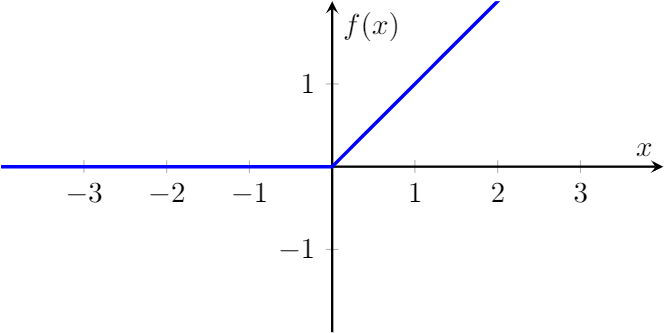
\includegraphics[width=0.3\textwidth]{Chapitre1/figures/relu.png}
  }
  \subfigure[Tan hyperbolic activation function]{
    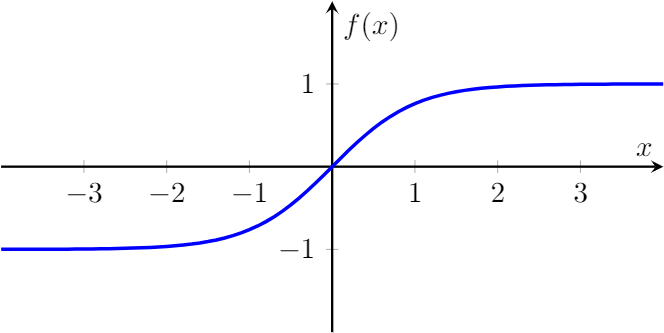
\includegraphics[width=0.3\textwidth]{Chapitre1/figures/Tanh.png}
  }
  \subfigure[Sigmoid activation]{
    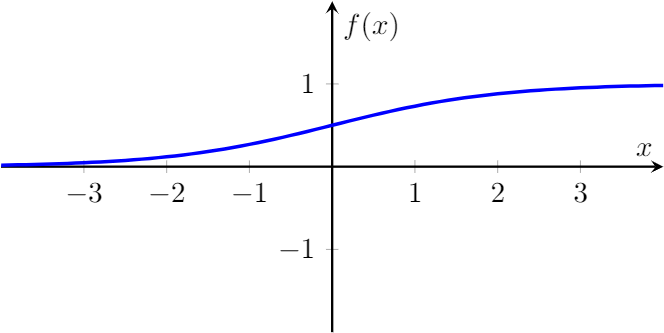
\includegraphics[width=0.3\textwidth]{Chapitre1/figures/sigmoid.png}
  }
  \caption{Relu, Tan hyperbolic function, and sigmoid activation function response.}
  \label{fig:multiple-figures}
\end{figure}


\subsubsection{Hyper-parameter Fine Tuning}% rephrase the title

Hyper-parameter tuning involves adjusting specific parameters in a machine learning model to improve its performance on a given dataset. These hyper-parameters, which are set before training the model, are not determined by the data and can include options like the learning rate or the number of hidden units in a neural network. There are different methods for tuning hyper-parameters, such as manually adjusting them and evaluating the model's performance, using a grid search to test all possible combinations of hyper-parameters, or sampling random combinations using random search. While hyper-parameter tuning is crucial for maximizing a model's performance, it can be time-consuming and resource-intensive.


\subsection{Network Regularization}% rephrase the title

Regularization is a technique used in machine learning models, especially neural networks, to prevent over-fitting. Over-fitting occurs when the model is too complex and has too many parameters, fitting the noise or random variations in the training data rather than the underlying pattern. This can lead to poor generalization performance for new unseen data.
We used two most commonly used regularization techniques: Dropout and batch normalization. 

Dropout \cite{srivastava2014dropout}  is a technique used in neural networks to prevent over-fitting by randomly "disabling" or dropping out a subset of the neurons during training. During training, randomly a fraction of the activations of the hidden units to zero, typically done with a probability of around 0.1 to 0.5. The probability of dropping out of the activation of each hidden unit is randomly sampled for each epoch of training. This forces the network to learn more robust features that are useful in different contexts, reducing complexity and improving generalization. During test time, all neurons are used but the activations are scaled down to compensate for the dropout rate used during training. Dropout is commonly used in combination with other regularization methods and has been shown to be effective in deep neural networks.

Batch normalization \cite{ioffe2015batch} is a technique used to speed up the training of deep neural networks and improve their ability to generalize. It works by normalizing the activations of neurons within layers for each mini-batch during training. Neuron activation values are typically distributed around a mean and vary in magnitude. This can cause problems in the optimization process. This is because the gradient of the weights can be very small or very large, depending on the range of activations. This can slow down training and makes the gradient disappear or explode. Batch normalization addresses this problem by normalizing neuronal activations so that each mini-batch has a mean and unit variance of zero. This results in a stable distribution of activations, more consistent gradients, faster training, and better generalization. Batch normalization is usually applied after linear transformations of activation and before nonlinear activation functions. 

\subsection{Evaluation of sound classification model}
Evaluating the performance of a proposed method is essential to determine its effectiveness. This evaluation should use metrics that reflect the real-world application of the method. Using standardized performance metrics makes it easier to compare and measure the progress made by the proposed method. 

\subsection{Performance Metrics}

To evaluate the performance of the ESC system, a performance metric is calculated using the binary detection outputs and the target outputs for a test or evaluation set. Commonly used performance metrics for ESC include \textit{accuracy}, \textit{precision}, \textit{recall} (also called the true positive rate), \textit{F1 score}, \textit{error rate}.  For polyphonic sound event detection, metrics such as accuracy are less effective to evaluate the performance, and error rate is generally used. Discussed in more detail in \cite{mesaros2016metrics}.

To evaluate the performance of the ESC system, a set of intermediate statistics, including true positives, true negatives, false positives, and false negatives, are calculated. These statistics can be used to calculate performance metrics at either the segment or event level.

A true positive is when both the reference and system output show that an event is happening during a specific time period. A false positive is when the reference says that an event is not happening, but the system output says it is. A false negative is when the reference says an event is happening, but the system output says it is not. True negatives are when both the reference and system output shows that an event is not happening. The total number of true positives, false positives, false negatives and true negatives are represented as TP, FP, FN, and TN, respectively.

\subsubsection{Accuracy}
Accuracy is a measure of the classifier's performance, calculated as the percentage of correct predictions made by the classifier out of the total number of predictions. It indicates how often the classifier is able to correctly identify the class of an input sample.

\begin{equation}
\label{eq:accuracy}
    ACC = \frac{TP + TN}{TP + TN + FP + FN}
\end{equation}

\subsubsection{Precision}
Precision is a measure of the accuracy of the detection made by the system. It is calculated as the ratio of the number of correctly detected examples to the total number of detection made by the system.

\begin{equation}
\label{eq:precision}
    P = \frac{TP }{TP + FP}
\end{equation}


\subsubsection{Recall}
Recall, also known as sensitivity or true positive rate, is a measure of a classifier's performance that indicates the proportion of positive instances that were correctly identified by the classifier. 

\begin{equation}
\label{eq:recall}
    R = \frac{TP}{TP + FN}
\end{equation}


\subsubsection{F1 Score}
The F1 score is a measure of a classifier's performance that combines precision and recall. It is calculated as the harmonic mean of precision and recall, with a higher score indicating better performance. The F1 score is defined as:

\begin{equation}
\label{eq:f1score}
    F1 = \frac{2 . P . R}{P+R}
\end{equation}

The F1 score is useful for evaluating the performance of a classifier because it can be applied to both single-label and multi-label classification tasks and considers both precision and recall equally. However, the F1 score does not take into account true negatives in its calculation.


\subsection{Cross Validation}
\label{cross_validation}
Cross-validation is a statistical method used to evaluate the performance of a predictive model by partitioning the original sample into a training set to train the model, and a test set to evaluate it. Cross-validation is an important aspect of comparing and reproducing results in experiments. It is important to carefully set up the cross-validation procedure to ensure that all classes are represented in each fold, as missing classes can result in errors in the calculation of some performance metrics \cite{sechidis2011stratification}. The model is trained on the training set and then tested on the test set. This process is repeated a number of times, with each partition serving as the test set once as depicted in Figure \ref{fig:crossvalidation} \cite{scikit-learn_cv}. The average performance across all iterations is used to assess the model's performance. It is important to treat the cross-validation folds as a single experiment and only calculate the final metrics after testing all the folds. Cross-validation helps to reduce the risk of over-fitting, as the model is trained and evaluated on different data each time. It is a widely used technique for model selection and evaluation.




\begin{figure}[htbp]
   \begin{center}
      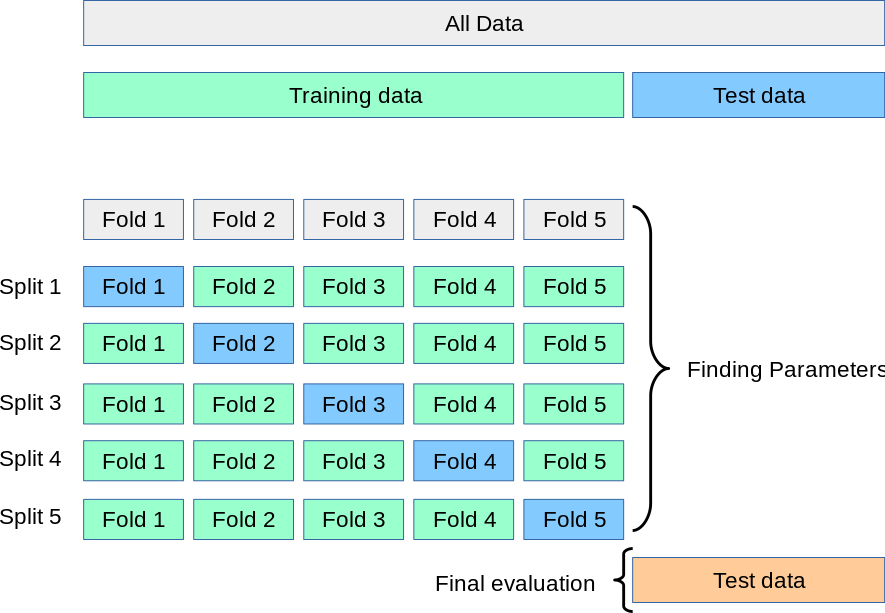
\includegraphics[width=0.8\linewidth]{Chapitre1/figures/grid_search_cross_validation.png}
   \end{center}
   \caption{ Multi fold cross-validation setup.}
   \label{fig:crossvalidation}
\end{figure}






\section{Datasets} % add graphs and tabels for the datasets
\label{chapter:backroundDatasets}
The dataset used to train and evaluate the ESC method should be diverse and representative of the range of ESC tasks it is intended to handle. This dataset can be created using sounds recorded in real-world environments and annotated manually, or by synthesizing sounds using individual sound events and mixing them to mimic real-world conditions. Synthesizing the dataset has the advantage of providing more accurate annotations, but it can be challenging to create sound event mixtures that accurately simulate a real-world recording.

The database consists of the audio recording and their associated labels. There are two types of labels that describe the granularity of the labels: strong labels and weak labels. In strong labeling, the desired sound and its time stamp are both present, for example, in an audio recording the time stamps of the start and end of the dog bark is presented along with the label. In weak labeling, only the general label is present without any information about the locality of the sound event present in the audio recording. Obtaining strong labels is a difficult and arduous task and is required for overlapping sound events. In this thesis, weak-labeled sound databases are used. The databases are described in the following section. The usage of these datasets for the development of proposed methods is discussed in the experimental section of the following chapters.


\subsection{Acoustic Scene Classification Dataset} %DCASE 2018 Task1A
Detection of an acoustic scene has been considered a complex problem by the research community for several years, and various efforts have been dedicated to solving this issue. Acoustic scenes contain acoustic events in a particular environment such as metro stations, airports, train stations, etc.  Classifying these categories becomes complex due to the similar nature of the sound events occurring in those environments. To solve this issue, the Detection and Classification of
Acoustic Scenes and Events (DCASE) provided a dataset that contains audio recordings of 10 different categories: airports, indoor shopping malls, metro stations, pedestrian streets, public squares, streets with a medium level of traffic, traveling by train, traveling by bus, traveling by an underground metro, and urban park (TUT Urban Acoustic Scenes 2018 dataset) \cite{Mesaros2018_DCASE}.

\subsection{Low-Complexity Acoustic Scene Classification Dataset } %DCASE 2020 Task1B

This dataset is provided by the DCASE community \cite{Mesaros2018_DCASE} and contains three categories. The dataset comprises  recordings from 12 European cities in 10 distinct acoustic scenes. The 10 different categories are then divided into three separate categories as follows: 
\begin{itemize}[label=$\cdot$]
\item {Indoor scenes: airport, indoor shopping mall, and metro station;}
\item {Outdoor scenes: pedestrian street, public square, a street with a medium level of traffic, and urban park;}
\item {Transportation-related scenes: traveling by bus, traveling by tram, traveling by underground metro.}
\end{itemize}

The audio signal is recorded at 48kHz and in 24-bit in a binaural format using only one recording device. The dataset is divided into two categories: the development set and the evaluation set. Due to the unavailability of the labels of the evaluation set, the system was evaluated  on the development set only. The development set contains 40 hours of audio recordings divided into a training set and a test set. Each audio file is 10 seconds long. The baseline system \cite{kumari2019edgel} is evaluated using the development set by log Mel filter bank energy features. 


\subsection{Urbansound8k}

Urbansound8k is a dataset containing 10 different classes and 8732 short-duration (less than or equal to 4 seconds) files \cite{salamon2015unsupervised, piczak2015environmental}. The collection is composed of environmental sounds such as air conditioners, car horns, playing children, dog bark, drilling, engine idling, gunshot, jackhammer, siren, and street music. Recordings are available in 10-fold cross-validation and recorded at 22.05KHz sampling frequency. 

\subsection{Custom Database}

 The audio recordings are collected from FreeSound \cite{10.1145/2502081.2502245} from several contributors. Each recording was registered by a different publisher and with different locations, lengths, equipment, and sampling rates. The recordings are gathered for four categories, i.e., rain, wind, car passing, and human walking. The recording's sampling rates were from 44100 Hz to 96000 Hz. The database was processed to obtain uniform characteristics. Ten-second audio files were extracted with a sampling rate of 441000 Hz, resulting in 750 files of 10-second length with a total duration of 125 minutes for each recording\cite{ahmed2021sound}.
 
